\documentclass{OUP-EJ}

% OTHER PACKAGES
\usepackage{graphicx}
\usepackage{amsmath}
\usepackage{amsfonts}
\usepackage{amssymb}

\begin{document}

\title[Populist Ideology, Policy and the Real Economy]{Populist Ideology, Policy and the Real Economy: Explaining Economic Growth in Populist Regimes}

\author[1]{Ege Asutay}

\author[2,*]{Christopher Ball}

\author[3]{Andreas Freytag}

\affil[1]{Friedrich Schiller University Jena, Germany (ege.asutay@uni-jena.de)}

\affil[2]{Quinnipiac University, Connecticut, USA; Corvinus University Institute for Advanced Study, Budapest, Hungary (christopher.ball@qu.edu)}

\affil[3]{Friedrich Schiller University Jena, Germany; University of Stellenbosch,  South Africa; CESifo Research Network (andreas.freytag@uni-jena.de)}

\corres[*]{christopher.ball@qu.edu}



\begin{abstract}
We argue that the classic populist ``walking stick'' pattern---an early boom of high growth and low inflation followed by stagnation and high inflation---can arise even without fiscal or monetary irresponsibility. In an open-economy endogenous growth model \'a la \cite{Romer1990}, reallocating labor from ``elite'' research jobs to manufacturing, as encouraged by populist ideology, boosts output temporarily but slows productivity growth, triggering a bust, inflation, and trade deficits. Using TWFE and PVAR estimations on late 20th-century populist and non-populist governments, informed by \cite{FunkeEtAl2023}, we find empirical support for this real-sector mechanism.
\end{abstract}

\keywords{populism; macroeconomic policy; economic growth; misallocation}

\subjclass[2025]{E02, N10, O43}

\thanks{Acknowledgements: We thank participants at the February 2025 PEDD-Workshop in M\"{u}nster, Germany, the March 2025 Seminar Participants in the University of Stellenbosch, Stellenbosch, South Africa, participants at the 2025 European Public Choice Meetings and at the 2025 Annual Public Choice Society Meetings.
}

\maketitle


\section{Introduction}\label{isect1}
The rise in populism in recent years has led to a renewed interest in understanding the implications of populist politics. Traditionally, the macroeconomics of populism has followed the views elaborated by \cite{DornbuschEdwards1990} who promote the view that populist governments pursue pro-growth policies by ignoring intertemporal budget constraints.  This then explains their historic tendency to over print both money and, when possible, bonds, leading to boom-bust cycles, inflation and currency crises when exchanges rates are fixed. The result is that, historically, populist policies have led to what \cite{BallFreytag2019} call walking stick – i.e., an inverted J-curve – results of a temporary GDP boom followed by long-term output decline with rising inflation.  Nothing in the traditional story, however, links those policies to populist ideology, \textit{per se}.

This paper remedies that by providing a real-sector policy that follows from populist ideology and also generates the walking stick output pattern. When combined with reasonable monetary policy, it also results in the sort of high inflation, current account deficits and currency depreciations observed historically but without the need to violate intertemporal constraints. We do this in a modified \cite{Romer1990} endogenous growth model of an open economy with money. 

\begin{figure}[t!]
    \centering
    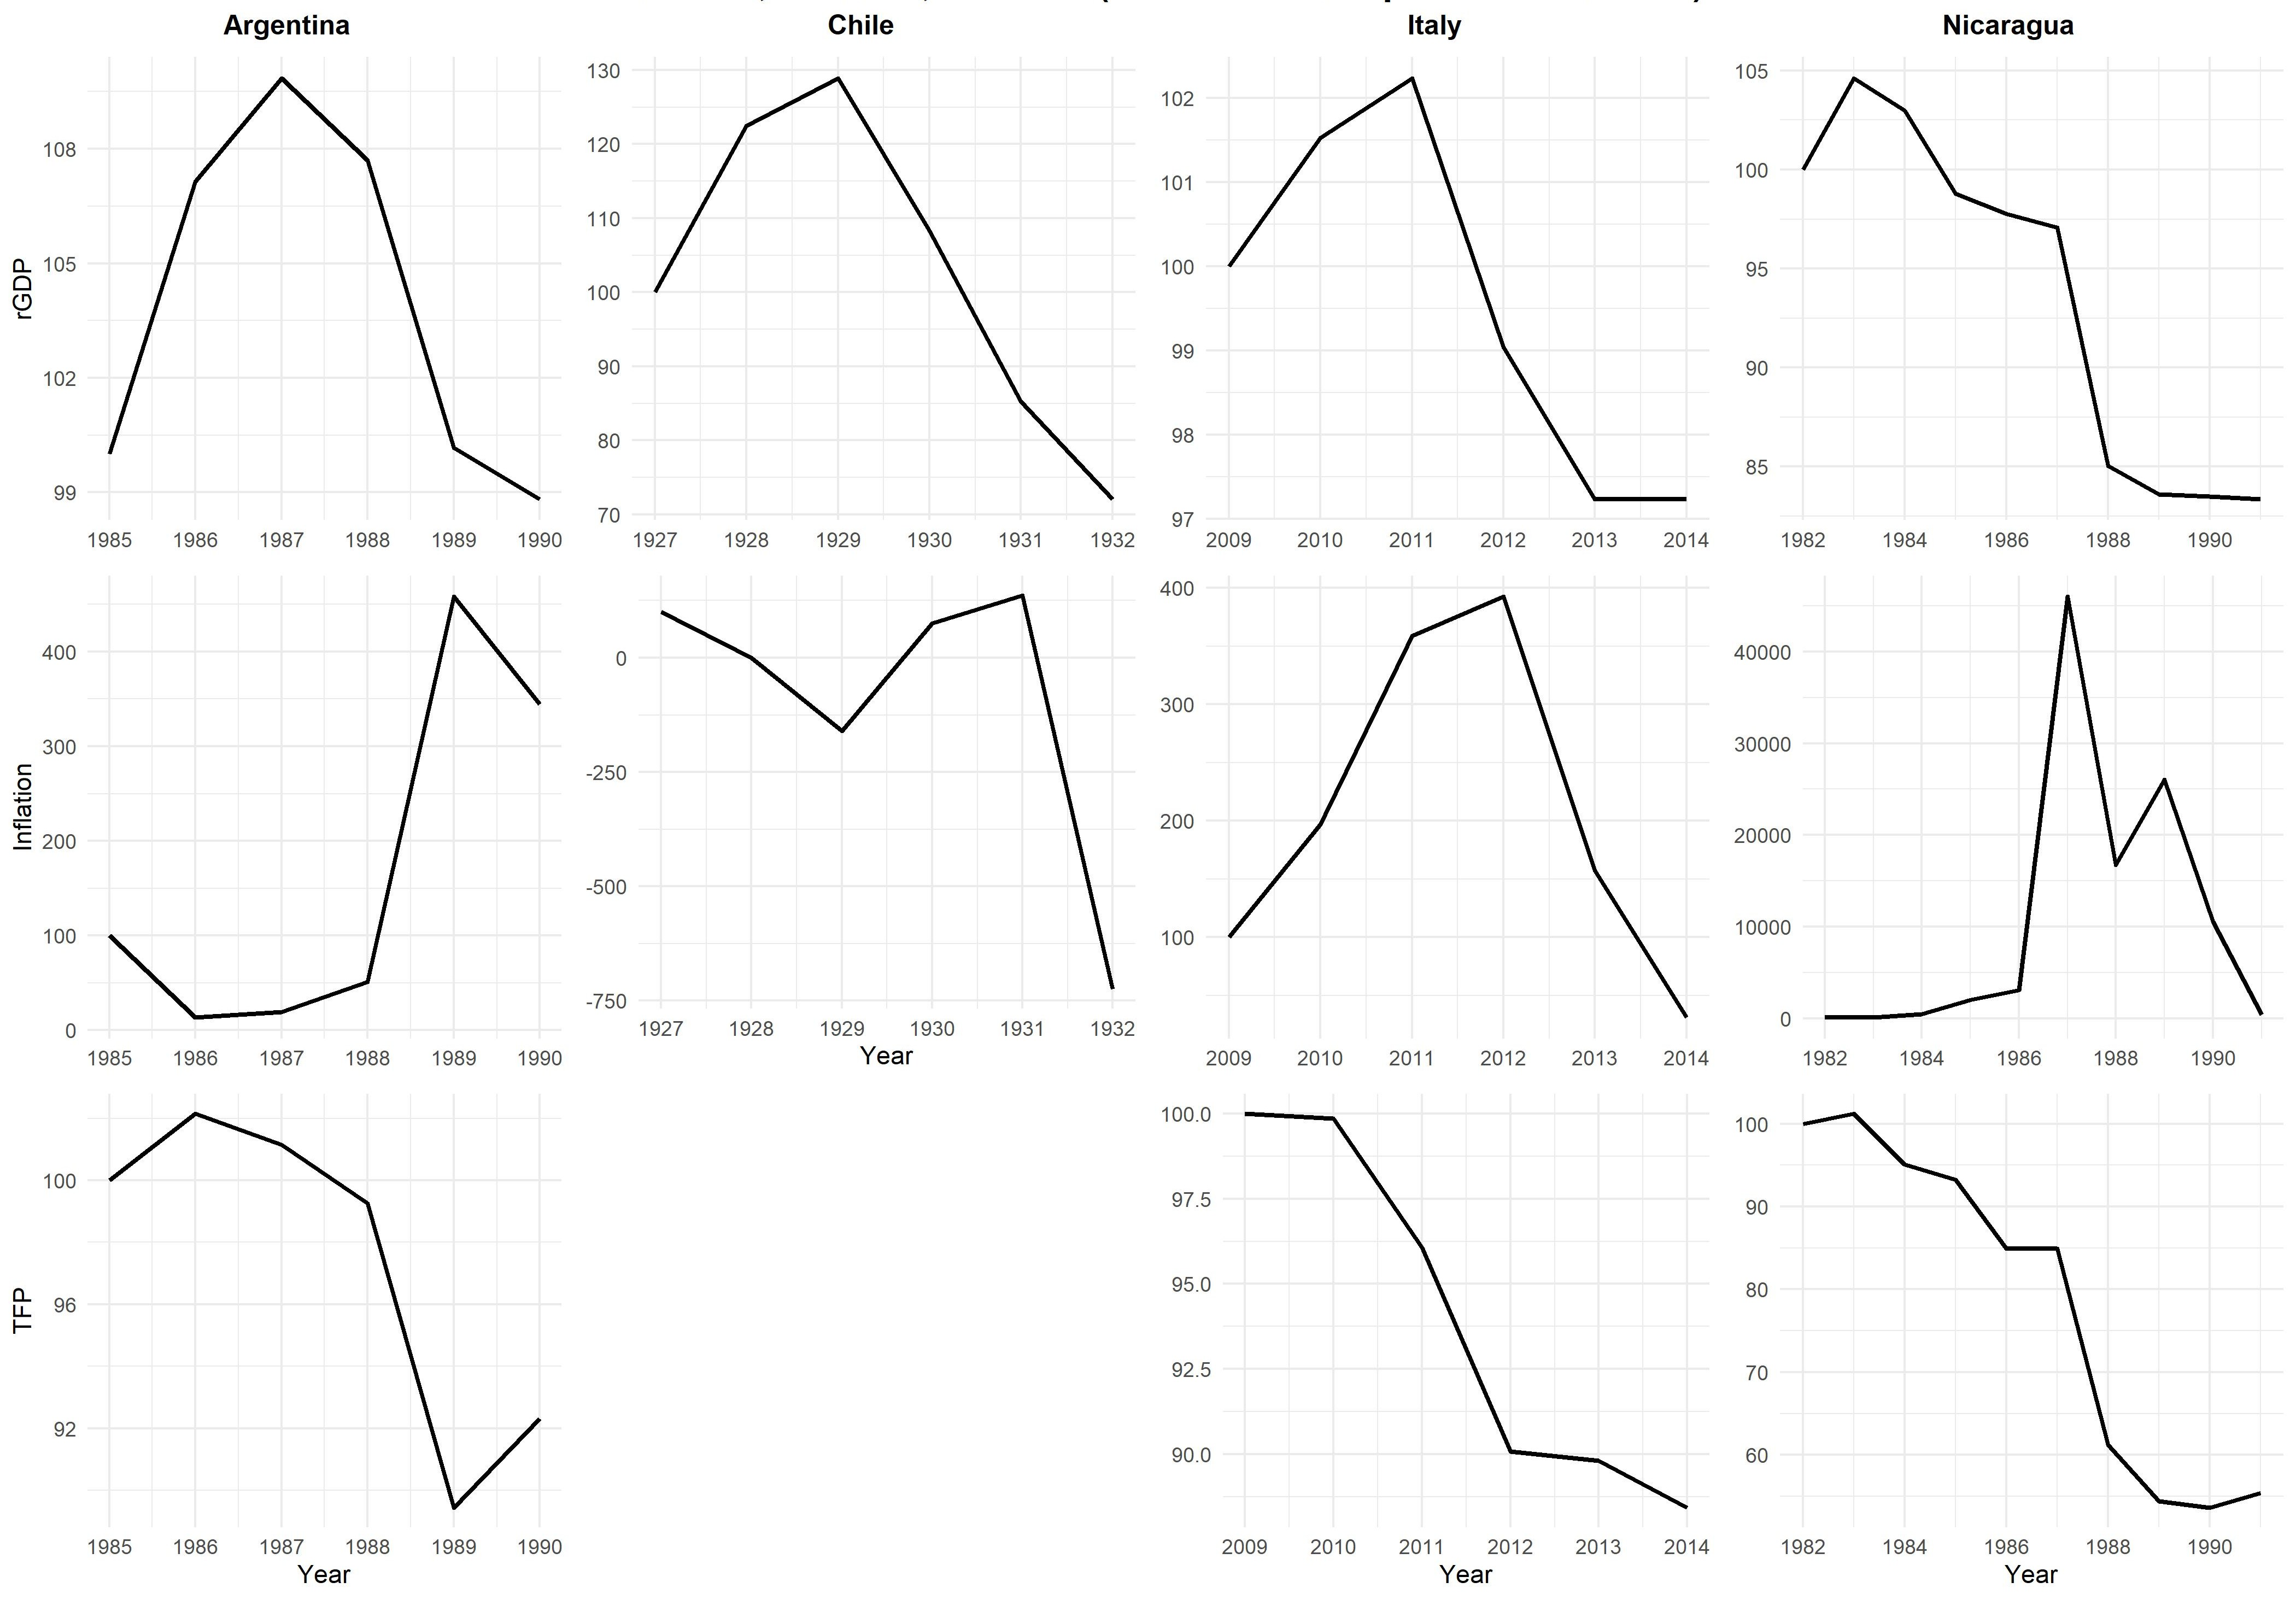
\includegraphics[width=\textwidth]{AllCountries_WS.jpeg}
    \caption{Populist Walking Stick Episodes (Start Date = 100)}
    \label{fig:intro_WS}
\end{figure}

Figure (\ref{fig:intro_WS}) presents four historical examples of walking sticks that occurred under populist governments across space and time. The countries are organized alphabetically and in each case the variable analyzed was normalized to 100 at the start of the period. Each case was also selected because it starts with a populist government in power.  The four cases are Argentina 1985-1990, Chile 1927-1933, Italy 2009-2014 and Nicaragua 1982-1991.  We do not have TFP data prior to 1960 and thus none for the Chilean example.  In all cases we see the basic pattern that we identify as a walking stick: a boom-bust cycle of GDP where the bust is longer than the boom, declining TFP and eventual inflation.  The Italian case overlaps with the Great Financial Recession and an austerity package that started in 2011. Nevertheless, the time period is under the populist governments of Berlusconi followed by Salvini and their policies.

This model and structure give us a natural context in which to consider populist policies. In particular, we focus on the aspect that the recent populist research has identified as central to all populist ideologies across time and geography: an “us versus them” and an “anti-elite” view of the world (see \cite{KaltwasserTaggart2015}, \cite{WysockiFreytag2024} and others). In our model, it seems natural that the local populist regime would identify workers in the research sector as the ``elite", or ``them”, and workers in manufacturing as ``us”. We then consider one possible populist, anti-elite policy: moving moves workers out of the “elite sector” of the economy. This generates an initial boom as labor enters the final goods sector and a long-term bust since less research is being produced over time.

The policy approach is intended as an analogy to capture the notion that populist policies can re-allocate resources along ideological lines in a way that can both generate an initial boom and also cause long-term decline due to decreased efficiency (here, declining technology).  Both traditional and modern populists have targeted ``elites/them" in higher-education, for example.  In Chile from the 1970s' Allende regime through Pinochet's famous employment of “the Chicago boys", fights over elites in intellectual leadership roles played a large part in government plans and economic policy \cite{Edwards2023}.  In the 2010's, Hungary's Victor Orb\'an forced the “elite” Central European University out of Hungary despite it being Hungary's best internationally ranked university (see \cite{NYT2018}).  Most recently, the Trump 2025 agenda plans to close the US Department of Education in line with the populist MAGA movement's efforts to both reshape the economy and also take it back from “out-of-touch elites” \cite{TrumpGOP2024}.  Interestingly, both modern populist examples perhaps the negative consequences as well since both took additional steps also to enhance productivity in the US's case \cite{TrumpGOP2024} and improve the remaining university in Hungary's \cite{CNN2021}.

Our work also relates to the growing research on misallocation and its macroeconomic effects (e.g. \cite{Reis2013}). This literature explores how microeconomic misallocations result in depressed or distorted macroeconomic outcomes. There is surely a wide range of real-world populist misallocation policies that we believe would have similar effects to the ones in our model. For example, tax policy could be used to discourage/punish workers in the elite sector, various ``us" sectors can be subsidized, or similar results could result from specially constructed tariff policies. Because our model is the first, to the best of our knowledge, to attempt to model the reallocative policies that are uniquely identified with and inherent to populist ideology, we made every effort to keep the model tractable and clear. Moving labor is as direct as we can be and allows us to consider one other aspect that naturally occurs: maintaining popular support and maximizing the economic boom.  In particular, we assume that populists are placed in office in part because of a belief that their policies will lead to economic growth. This has long been recognized as a reason for their support, \cite{DornbuschEdwards1990}. In our model, then, populist policy makers can reallocate labor to maximize the boom period, thereby delaying the start of the economic decline and their eventual removal from office. 

The remainder of the paper is organized as follows. We first summarize the literature including a definition of populism. We then present the model. Our baseline analysis shows that real GDP growth first increases, then decreases over a populist president’s time in office while non-populists do not follow this pattern. Moreover, we observe the opposite for consumer price inflation. Both these findings are in line with our broader walking stick hypothesis. We then test the walking stick hypothesis on a unique panel data set of 62 countries spanning 1970 to 2019. 

\section{Literature Review}

The rise of populism in recent years has led to a surge of interest in the causes of populism’s recent (re)emergence (see \cite{Inglehart2016}, \cite{Judis2016}, \cite{Margalit2019}, \cite{Rodrik2018a} and \cite{Rodrik2018b}). A less intensely asked question is what the likely effects of populism will be. Before we show the relevant literature dedicated to this question, we first summarize the literature’s contribution to a definition of populists which allows us to test our hypothesis empirically

\subsection{What defines a populist?}

There is now a vast literature attempting to define populist governments conceptually and identify them in reality. The problem is that populists run the political gamut from left- to right-wing and engage in a diverse range of policies commensurate with their left- or right-leaning views. For all of them to be recognized as populist, there must be some common non-economic elements. \cite{Kaltwasser2018} calls this an ideational approach.

In such an ideational approach, populism is defined based on two characteristics. First, populists distinguish between “us and them” (\cite{AlbertazziMcDonell2008}), with “us” including the populists themselves and the people, while “them” represents an allegedly corrupt domestic elite and/or foreign actors. Populists usually claim that only they understand the true public will (“\textit{volonté generale}“) (\cite{HouleKenny2016} and \cite{KaltwasserTaggart2015}; among others). The second characteristic of a populist politician (or party) is a certain dislike of liberal democracies and especially the necessity to compromise in such a pluralistic regime (\cite{Kaltwasser2018}).

A rather economic definition of populism suggests that populists use short-term oriented economic policies which protect the people from uncertainty and foreign threats (\cite{GuisoEtAl2017}). In the modern approach, \cite{AcemogluEtAl2013} argue that populists implement policies supported by a large share of the population that finally hurts exactly these supporters. The older literature focuses on populists’ preference for a mix of distributive and expansionary fiscal policies backed by protectionist policies to protect the population from the negative effects of this combination. This implies that they neglect macroeconomic constraints (see \cite{Sachs1989}, \cite{DornbuschEdwards1991}, \cite{Edwards2019} and \cite{GuisoEtAl2017}). This economic definition of populist bears the problem that it is not useful to test the economic consequences of populism empirically as it does not allow to select populist governments other than by ‘guilt’ (\cite{BallFreytag2019}). It is also rather likely that an economic definition may restrict the analysis to left-wing populists (\cite{Kaltwasser2018}). 

This leads to the question of who in the real world can be called a populist and who cannot. Today, populist governments range from far left to far right in the political spectrum which is different from the 1960s, 1970s and 1980s when populist governments – mainly prevalent in Latin America – were mostly located on the left end of the political spectrum \cite{Sachs1989} and \cite{DornbuschEdwards1990}. \cite{Weyland2001} presents a definition, conceptualization and categorization of different types of Latin American populists. His work is indeed groundbreaking for those who apply empirical models. 

Conceptually, populists clearly exhibit ``us versus them" rhetoric that is manifest in their policy actions such as redistribution from ``them/elites" to ``us" and also in a strong pro-growth agenda.  While traditional views emphasized static, leftist redistribution, we will argue this might also include reallocation of resources which we operationalize as a real-sector policy in our model. Additionally, the pro-growth emphasis traditionally implied primarily overly expansive fiscal and monetary policy, we will interpret this again as a real-sector policy. Hence the two views are combined in reallocating ``elites" away from the ``elite" sector in a way that also generates growth. To measure and identify populist regimes empirically, there are several options. \cite{FunkeEtAl2023} apply a zero-one dichotomy, and identify populist regimes based on the definition of \cite{Kaltwasser2018}. \cite{CelicoEtAl2024} use a different method. They build an index of populism based on machine learning.

\subsection{The Economics of Populism and The Walking Stick Synthesis}

Interestingly, populists’ general distrust of elites means that they do not tend to adhere to any specific economic school of policy thought. This makes it difficult to assign certain policies to populists and make predictions from populist polices to outcomes, as they seem to favor instead ``whatever works”. The literature is prone to this problem to a certain extent. Our paper is an attempt to solve this problem.

As mentioned above, the literature about ``why now” is larger than that about “what next”; we are interested in the latter. First, there is an older macroeconomic literature concluding that left-wing Latin American populism caused macroeconomic problems, namely balance of payments crises and economic collapse. \cite{Sachs1989}, \cite{DornbuschEdwards1990} and \cite{DornbuschEdwards1991} all detected a boom-bust pattern in GDP, which also in later papers has been associated with populist regimes. It is interesting to note here that such policies are not entirely restricted to populists as defied by the political definition above – democratic governments without populist properties have also followed this policy pattern.

\cite{DornbuschEdwards1990} and \cite{DornbuschEdwards1991} make an interesting distinction of various phases of political and economic development under populism, which is relevant for our analysis of a walking-stick pattern. Phase 1 is the period before the populist leader gains power. In Phase 2, the initial boom begins and makes populist policymakers appear successful. In Phase 3 expansionary demand runs into bottlenecks, a lack of foreign exchange, and capital flight. This then leads to Phase 4, described as the prelude to collapse and characterized by shortages, increased capital flight, and extreme acceleration of inflation. Finally, in Phase 5 a new government enters to clean up the mess. \cite{BallFreytag2019} base their analysis on these papers and show that populist governments in Latin America by and large have created a pattern best described by a walking stick (an inverted J-curve). The first authors of the late 1980s and early 1990s don’t call it such but can be recognized as foundational in this form of macroeconomic study of populist economic policy formation and its generally disastrous results. \cite{BallFreytag2019} try to test this time line by distinguishing different periods of a populist’s term to identify the walking stick. However, the method they use is not fully convincing, as they split populists’ terms in Latin America between 1975 and 2012 – regardless of their duration – into two halves. In the first half, inflation was lower and growth was higher than in the second half. 

\cite{Edwards2019} reviews his older work and introduces microeconomic policies also pursued by populists. He thereby sees a changing trend, identifying Classical (pre 1990) and New Populist (post 1990) regimes in Latin America; all in all he identifies 15 populist regimes. In his view, the Classical Populists tend to be “macroeconomic populists”, because they rely on monetary policy to finance their fiscal policies. By contrast, he argues that New Populists seem to be more “microeconomic populists” with a focus on regulation, protectionism and other public sector policies. For our analysis, this is an important extension to the first papers.    We build on the effort to draw more subtle distinctions by identifying populist regimes that primarily rely on the original \cite{DornbuschEdwards1990} policies of expansive monetary and fiscal policy as Dornbusch-Edwards populists (also referred to as High-M2 populists) and those that rely instead on real-sector reallocations as real-sector populists (also referred to as Low-M2 populists).  Our real-sector populists are more in the vein of the \cite{Edwards2019} microeconomic populists.  Of course, the categories are not mutually exclusive.  We use these distinctions to help organize the data in our empirical analysis.

Using the synthetic control method, \cite{FunkeEtAl2016} construct a comprehensive dataset of 60 populist regimes over 120 years (between 1900 and 2020) and show that populist governments reduce economic growth significantly – 15 years after populist governments took office, GDP/capita was 10 percent lower than it could have been in the very countries under a non-populist regime. These results are confirmed in recent paper by \cite{ChuangEtAl2024} using exactly the same data and recoding populists.

Of course, such a simple pattern (macroeconomic populists until 1990, microeconomic ones thereafter) does not account for the diversity of regimes on the one hand and their common attitude towards established parties and so-called elites, on the other. For instance, the Polish PIS government in the late 2010s and early 2020s has rather created a typical macroeconomic problem, as \cite{WysockiFreytag2024} have documented in their analysis. Using the concept of fiscal sustainability, they show that the PIS government used short-term macroeconomic policies with a redistributive element, which reduced fiscal sustainability in the aftermath of these policies.

Interestingly, \cite{Rodrik2018a} argues that populist policymakers can pursue welfare enhancing policies if non-populists use rule-bound policies – such as the global trade order – to privilege special interests at the expense of the broad population, which first gives rise to a populist government that subsequently abandons the rule and corrects the distribution problem – this can indeed lead to the walking stick pattern.

However, not only did macroeconomic problems emerge from these policies, but also inequality and social conflict, as described by \cite{Sachs1989} who analyses populist policy cycles in Argentina (1946-49), Chile (1971-73), Brazil (1985-88), and Peru (also 1985-88). He thereby extends the discussion to show how social conflicts could interact with distributive goals and fixed exchange rate regimes to create a negative “populist policy cycle” \cite[p.15]{Sachs1989}. He further argues that these economic policies had disastrous results. 

From our perspective, the political science and political economy literature on populism is highly relevant as it has recently started to study both the causes and effects of populism’s resurgence. One vein has worked on understanding the causes of populism ranging from the role of distrust in public institutions \cite{Doyle2011} to economic insecurity \cite{FunkeEtAl2016}.  Another vein has looked at the effect of populism on public institutions from the general quality of democracy in terms of rule of law, the judiciary and so on to economic “institutions” like the degree of freedom \cite{HouleKenny2016}. \cite{BastosEtAl2023} use these rather historical results in Latin America to come up with an interesting extension which adds a highly negative attribute to populist leaders. The longer they govern, the more they become like stationary bandits in the \cite{Olson1993} sense. That is, they exploit the country to their personal benefit. If term limits restrict them, left wing populists intensify the exploitation and behave like roving bandits. 

This is in line with three newer contributions to the literature that can be seen in the tradition of public choice. \cite{Shmuel2025} shows that populists drive political business cycles, i.e. a boom-bust cycle spurred before general elections, more than non-populist governments. \cite{SassoEtAl2021} theoretically show that populists hire mostly opportunistic bureaucrats who feign loyalty to populism in exchange for competent career administrators. This renders the quality of public service sub-optimal. In this context a new theoretical contribution by \cite{SzeidlSzucs2025} shows that populists may have an interest to harm exactly those interests which they pretend to focus on. By establishing an alternative reality and blaming the ‘old elites’ for the populists’ failures, the latter can reduce own accountability.

Our contribution is based on but goes beyond the literature as we formulate our main hypothesis, claiming that populist governments produce a walking stick, i.e. a boom first and subsequently a bust. In order to develop and test this hypothesis, we use the political definition of a populist based on \cite{Kaltwasser2018} and a binary measure of populist government based on this definition as in \cite{FunkeEtAl2023}.   This requires first a solid theoretical framework.

\section{The Model}
We modify a \cite{Romer1990} endogenous growth model to be a small open economy with money. Households can borrow internationally at a constant world real interest rate which allows for non-zero current accounts. The government prints money which it transfers to households. 

The model has a final goods manufacturing sector and a research sector. There is a fixed supply of total labor which individuals allocate freely across the two sectors. Final goods manufacturing combines capital and labor with the currently available stock of technological knowledge. The research sector combines labor with the current stock of technological knowledge to produce new additions to that stock. The economy grows by producing new knowledge which constantly enhances the productivity of capital and labor in the final goods sector.

Our model adds depreciation to the stock of technology in the same way that capital depreciates. The idea is that, if not maintained, knowledge is slowly lost.  We are not alone in such a modification.  \cite{MankiwRomerWeil1992}, an early example, modify an endogenous growth model to include a depreciation rate on the stock of human capital.  They explain (p. 416) “we are assuming that human capital depreciates at the same rate as physical capital. \cite{Lucas1988} models the production function for human capital as fundamentally different from that for other goods. We believe that, at least for an initial examination, it is natural to assume that the two types of production functions are similar.”

More recent research focuses on using depreciation to merge endogenous growth models with DSGE-type models to study the effects of misallocation. \cite{DouEtAl2024} call their depreciation rate a ``patent obsolescence rate" and use it to modify a \cite{Romer1990} model to study endogenously emerging capital misallocation that affects growth. They are able to show larger and longer-term effects from misallocation than are found in other misallocation growth models such as \cite{Moll2014}. 

\cite{CominGertler2006} use such a framework to explain both high- and medium-frequency variation in data as well as endogenous movements in productivity to explain persistence in these fluctuations which they call ``medium-term business cycles".   \cite{MoranQueralto2018} show how monetary policy can affect R\&D and thus have longer-term output effects than found in normal New Keynesian models. \cite{AnzoateguiEtAl2019} show how financial crises can similarly lead to longer-run productivity and growth declines and, in their case, slower recoveries.

Our model uses this modeling approach to study the effects of a policy that misallocates labor for political reasons.  The government in our model follows its populist ideology to restructure the economy. It comes to office promising to pursue two classic populist goals: (1) the punishment of elites and (2) the achievement of higher economic growth.  Jobs are reallocated from “elite-occupations” in the research sector to the manufacturing sector. This re-allocation leads to a temporary boom followed by a decline in real output, as the reduction of research activities reduces productivity growth. This produces a walking stick pattern for real GDP.

The real-economy walking stick drives all the other results without the need for government to try to break intertemporal budget constraints. In this environment, a basic real-world monetary policy that targets a long-run inflation rate by keeping money growth consistent with the target, given backward-looking estimates of trend GDP growth, will over print money relative to output in the medium-run causing a bout of inflation.

\subsection{Solving The Model}

We employ a modified \cite{Romer1990} model in discrete time.  It is modified in three ways. First, we assume that technological knowledge depreciates at a constant rate. Second, we assume the economy is a monetary economy which also requires formally modeling the government's budget constraint and defining a monetary policy. Finally, we assume this is a small open economy.

\subsection{Households}

A representative household maximizes discounted lifetime utility over consumption, $c_t$, and real money balances, $m_t$, that is assumed to be separable in its arguments. 

\begin{equation}
    \label{utility}
    \sum_0^{\infty} \beta^t u(c_t,m_t)
\end{equation}

where $\beta$ is the subjective discount factor.  Utility will be assumed logrithmic so that $u(c_t,m_t)= \log (c_t) + \log (m_t)$.

Households maximize equation (\ref{utility}) to subject to the following real, flow budget constraint

\begin{equation}
    \label{real budget}
    \frac{m_{t-1}}{1+\pi_t}+ (1-\delta_k) k_{t-1} + (1+r^*)b_{t-1} + y_t + v_t  = b_t + k_t + c_t + m_t.
\end{equation}

Households enter each period with real money balances from the previous period, $m_{t-1}$, capital remaining after depreciation, $(1-\delta_k)k_{t-1}$, and earn international returns, $1+r^*_{t-1}$, on the stock of real one-period internationally traded bonds denominated in foreign currency, $b^*_{t-1}$, which are evaluated in domestic currency by the nominal exchange rate, $E_t$, which is defined as domestic relative to foreign currency. They sell final goods, $y_t$, and receive real net transfers from the government, $v_t$, which also serve as the mechanism by with the government adds money to this economy.  Individuals then purchase new international bonds worth, $b^*_t$ , capital, $k_t$, spend on consumption of the final good, $c_t$, and acquire additional real money, $m_t$, to carry into the next period. Time subscripts are such that $t$ denotes a choice in period $t$.  Hence, stocks yielding benefits in period $t$, such as capital, international bonds, and technology are pre-determined and have subscripts $t-1$.

The final goods production function follows \cite{Romer1990}, 

\begin{equation}
    \label{production fn}
    y_t = k_{t-1}^{\alpha}A_{t-1}^{1-\alpha}l_{1,t}^{1-\alpha} 
\end{equation}

Production combines current manufacturing labor, $l_{1,t}$, with pre-existing capital, $k_{t-1}$ and technology, $A_{t-1}$.

Total labor, $L$, is fixed and allocated between work in the manufacturing sector, $l_{1,t}$, and in the ``elitist" research sector, $l_{2,t}$.  That is, $L=l_{1,t}+l_{2,t}$.

The real budget constraint, equation (\ref{real budget}), production function, equation (\ref{production fn}), along with the equation of motion for the evolution of technological knowledge are the constraints households must consider in maximizing lifetime utility (\ref{utility}).  Technology evolves as follows,

\begin{equation}
    \label{tech accum}
    A_t=\theta A_{t-1} l_{2,t}+(1-\delta_A) A_{t-1}
\end{equation}

which says that total amount of technological knowledge at any date - to be employed in subsequent dates - is made up of new knowledge produced according to the linear production function, $\theta A_{t-1} l_{2,t}$ where $\theta$ is labor productivity in the research sector plus what is carried over from the past. But, we allow technological knowledge to depreciate over time as well.

\subsubsection{Capital}
The economy is open with perfect capital mobility (captured by interest parity) and world real rates are assumed constant, we can therefore combine optimality conditions (in Appendix equations (\ref{L_k}) and (\ref{L_b})) to obtain 

\begin{equation}
    \label{MPK=r}
    \alpha k_{t}^{\alpha-1}A_{t}^{1-\alpha}l_{1,{t+1}}^{1-\alpha} = r^*+ \delta_K
\end{equation}

which equates the marginal product of capital with the capital-depreciation-adjusted world real interest rate.  Time subscripts here reveal that the marginal product of capital, for capital being chosen today at time $t$ to be used in production tomorrow, must include an expectation of labor tomorrow, $t+1$.  In our simulations, labor in this sector, $l_1$, will be exogenously determined by policy makers using $l_2$ as a policy variable since $L=l_{1,t}+l_{2,t}$.

\subsubsection{Piece-wise Constant Consumption}
We assume that $\beta (1+r^*) = 1$ to avoid a steady state motive to borrow or lend internationally. This also implies that consumption will be piece-wise constant since the optimality conditions for consumption equation (\ref{L_c}) and for international bonds (\ref{L_b}) imply $u_{c_t}=\beta (1+r^*)u_{c_{t+1}}$ so that, for separable, logarithmic utility, $c_t = c_{t+1}=c$.

\subsubsection{Money Demand}
Money in utility yields the typical real money demand equation here which comes from combining equations (\ref{L_m}) with (\ref{L_c}) and (\ref{L_b}) along with the definition of nominal interest rates, $1+i_t=(1+r^*)E_t(1+\pi_{t+1})$.  Given log utility and the fact that consumption is constant we can write money demand,

\begin{equation}
    \label{m_d}
    m^d_t=c \left( \frac{1}{i_t}+1 \right).
\end{equation}

Given $M_t$, this equation determines the price level at each point in time.

\subsection{Government and Monetary Policy}

This is an open, monetary economy.  The government's primary job in this model is to manage monetary policy. It prints money, $M_t$ and transfers any surpluses to individuals via net transfers, $V_t \equiv P_t v_t$. 

Throughout we will assume that purchasing price parity (PPP) holds at all points in time and normalize the world price level to unity so that $P_t = E_t$.  Additionally, we assume uncovered interest parity holds and that world real interest rates are constant,$r*$, so that $1+i_t=(1+r*)(1+\pi_t)$ since constant foreign prices renders foreign inflation zero and PPP equates currency depreciation rates with domestic inflation.

The government's real flow budget constraint is

\begin{equation}
    \label{gov bc}
    v_t=\frac{\Delta M_t}{P_t}
\end{equation}

which can be written as $v_t=m_t - \frac{m_{t-1}}{1+\pi_t}$. We will assume that the government pursues a constant inflation target, $\pi^T$.  In steady state this implies a constant growth rate, $\mu_t=\mu$, of the nominal money stock.  In this case, $\mu_t = \pi_t$ which pins down the supply side of the money market and monetary equilibrium then obtains when $M_t^s / P_t \equiv m^s_t=m^d_t=c_t(1/i_t +1)$, given $M_t$.  Since we are not focusing on exchange rate policy, we assume a flexible rate regime and zero central bank international reserve holdings. Thus, equation (\ref{gov bc}) is also the consolidated government budget constraint for this economy.

\subsection{Balance of Payments}

Combining the household's and government's budget constraints yields the economy's aggregate resource constraint which, here, is the economy's balance of payments equation.  Combining equations (\ref{real budget}) and (\ref{gov bc}) yields

\begin{equation}
    \label{BoP}
    \Delta h_t=[y_t-c_t-\Delta k_t -\delta_K k_{t-1}]+[r^*(b_{t-1}+h_{t-1})] + [-\Delta b_t].
\end{equation}

The left-hand side term is the change in international reserves ($\Delta h_t$). The first bracketed term is the trade balance, the second, the income balance on both private and government holdings of real net foreign assets and the final term is the capital account ($-\Delta b_t$).

\subsection{Steady State}

We solve for steady state and use these values as the initial values for the variables in our simulations.  In steady state, $A_t = A_{t-1}=A_{ss}$ and thus drops out of equation (\ref{tech accum}), allowing us to solve for the steady state level of employment in the ``elite" research sector,  $l_{2,ss} ={\delta_A}/{\theta}$.  By our labor constraint, this implies that labor in the final goods sector is determined as well, $l_{1,ss}=L-l_{2,ss}$.

Since $A_{ss}$ drops out completely - as it would without depreciation as well - and isn't determined elsewhere in the model\footnote{It also drops out of optimality condition (\ref{L_A}) which is used instead to find the optimal amount of labor in the research sector outside of steady state.}, we treat it as a parameter. This is a feature of the \cite{Romer1990} technology accumulation equation.

In steady state, given $l_{1,ss}$ and $A_{ss}$, equation (\ref{MPK=r}) can be solved for the steady state level of capital which is $k_{ss} = \left[{\alpha}/(r^*+\delta_k) \right]^{\frac{1}{1-\alpha}}(A_{ss}l_{1,ss})$.  Given the steady state level of capital, along with the other previously determined steady state values, output is also determined as $y_{ss} = k^{\alpha}_{ss}A_{ss}^{1-\alpha}l_{1,ss}^{1-\alpha}$.

Given the above, steady state consumption is then found by solving for the aggregate resource - or balance of payments - constraint in steady state.  Doing so yields, $c_{ss} = y_{ss}-\delta_K k_{ss}$.

A constant money growth rule and the requirement that real money balances be constant in steady state yields $\mu_{ss}=\pi_{ss}$ which also pins down the rate of exchange rate depreciation in an open economy context with constant world prices, $\pi_{ss}=\varepsilon_{ss}$.  That in turns determines the steady state nominal interest rate, $i_{ss}=r^*+\pi_{ss}$. Given the above, real money balances in steady state are $m_{ss} = c_{ss}\left(1/i_{ss} +1 \right)$.

Finally, for an open economy, the trade balance in steady state is $NX_{ss} =y_{ss}-c_{ss}-\delta_k k_{ss} = 0$ which, along with our assumption of zero initial private or governmental holdings of international bonds $b_0=h_0=0$, implies the current account is also zero, $CA_{ss} = NX_{ss} - r^* (b_{ss}+h_{ss}) = 0$, as will be the capital account, $CA_{ss} = -KA_{ss}$.

\section{Policy Experiments and Simulations}

We start at date $t=0$ in steady state and assume a new, populist government comes to power.  The ``populist government" comes to office promising to pursue two classic populist goals: (1) the punishment of elites and (2) the achievement of higher economic growth. To achieve these, the government moves people from the ``elite" research sector into manufacturing.  During the boom phase, the policy will appear successful, achieving both populist objectives.

\subsection{The Core Walking Stick Mechanism}

The core walking stick mechanism moves workers from the ``elite" research sector into final goods production.  It has two primary effects that drive the walking stick pattern in output.  First, since production at any given time is based on existing stocks of technology and capital, the increase in labor unambiguously increases output upon impact by the marginal productivity of labor,

\begin{equation}
    \frac{\partial y_t}{\partial l_{1,t} }=(1-\alpha)k_{t-1}^{\alpha} A_{t-1}^{1-\alpha}(l_{1,t})^{-\alpha}>0.
\end{equation}

Second, since the policy simultaneously lowers labor in the research sector, it decreases the production of new technology causing a subsequent decline in technology and therefore, eventually, of output as well.  Using equation (\ref{tech accum}), the impact on new technology production of a change in research labor is

\begin{equation}
    \label{init drop in A}
    \frac{\partial A_t}{\partial l_{2,t}} = \theta A_{t-1}>0.
\end{equation}

For a decline in $l_{2,t}$, then, there is a decrease in the production of new technology equal to the amount of the marginal product of labor in this sector.

It's worth noting that these two effects are sufficient to cause a walking stick pattern, no matter the size of the initial decrease in labor in the ``elite" research sector.  The presence of technological depreciation means that any decrease in labor in this sector below its steady state level will cause a permanent decline in the stock of technology as it asymptotically approaches zero. At that point, output must also be zero regardless of capital or labor, $y_t=0 k_{t-1}^{(1-\alpha)} (l_{1,t})^{-\alpha}=0$.  The precise shapes of the transition paths depend on many factors but the walking stick outcome is fundamentally unavoidable after the initial change.

\subsection{Rationality}

To simulate the economic effects of such policies we cannot logically assume rational expectations. If individuals all formed expectations rationally in the traditional economic sense, they would account for the eventual bust period which leads to a zero technology, zero output, zero consumption steady state and would therefore never vote the populists in office in the first place.  The populists, likewise, would see the error of their ways prior to implementation and never implement or even propose such policies in order to get elected. But, in reality they do propose such policies, get elected, and have initial success despite the long-run failure.  The effects of this are what we want to study and assuming rational expectations would preclude such policies.

As a base case we assume agents form adaptive expectations over all endogenous variables. They do so in a way that applies a uniform weighting of historical information.  In this case, $E_{t_n} (X_{t_n+1})=\frac{1}{n} \sum_{i=0}^{n} X_i$ where $t_n$ is the date n-periods from initial steady state.  This fits our narrative the best in that the world starts in steady state with zero growth, populists enter power claiming both to punish elites and grow the economy.  Critics claim doom and gloom. Populists claim it will be a success.  Whom to believe is not clear \textit{ex ante}.

The only thing that is clear for sure is what policies the populists will implement. We therefore assume that the populists enjoy full credibility in terms of policy implementation.

To capture this, in each period, when determining the expected values of endogenous variables for the next period, all agents use the cumulative growth rate from all present and past periods as a best forecast. This matters not only for households but also for policy makers in setting monetary growth targets.  It implies that policy makers set monetary targets given expectations of trend output.  It therefore imposes consistent expectations for all agents across the economy.

It should be noted that how we handle expectations does not affect the core result that moving ``elite" labor out of the research sector leads to an initial boom and subsequent decline.  The walking stick pattern emerges under all expectations regimes - even rational expectations or, here, perfect foresight - via the core walking stick mechanism.  The different expectation regimes only affect the shapes of the time paths of the other endogenous variables as they respond to the populist-policy-driven walking stick.

\subsection{The path of consumption}

The path most affected by the (ir)rationality assumptions we make is that of consumption.  Consumption is piecewise linear in an open economy with a constant world real interest rate.  Under perfect foresight, this would mean that consumption would remain constant at its steady state level, only changing via a one-time jump upon announcement of new information that alters the steady state.

Since we don't use perfect foresight here, we allow consumption to remain constant at its initial steady state level throughout our base simulations.  As a robustness check we simulate cases where consumption jumps to its new steady state level (one where the research sector has no employees and technology has reached its minimum possible level). Because the core mechanism is independent of consumption the only notable difference is that when consumption jumps to its new, lower steady state level upon announcement the sudden drop in domestic consumption combined with an increase in output via the core mechanism generates a one-time trade surplus upon announcement of the new policy.

\subsection{Simulating Populist Policy Effects}

We model populist policy regimes as the government forcibly moving ``elites" out of the research sector and into the final goods sector.  How fast they reallocate labor is an additional choice.

One strategy would be to go ``all in" and move all the elites in the first period of office. Doing so would generate a large but short-lived initial boom.  Another strategy would be to implement the policy partially but repeatedly in order to get a smaller but longer-lived boom. We feel this is a likely policy in practice since, after confirming the initial success of their reallocation strategy, they would be inclined to repeat it.  This would also likely lengthen their time in office since it expands the period of perceived success.

Figure (\ref{fig:output_and_tech}) presents the simulated paths for output and technology under three example: (1) ``all at once" where all labor is reallocated from research to manufacturing, (2) ``fifty percent" where each period fifty percent of the current labor stock in research is reallocated, and (3) ``baseline" which extends the boom for as long as possible.

\begin{figure}[t!]
    \centering
    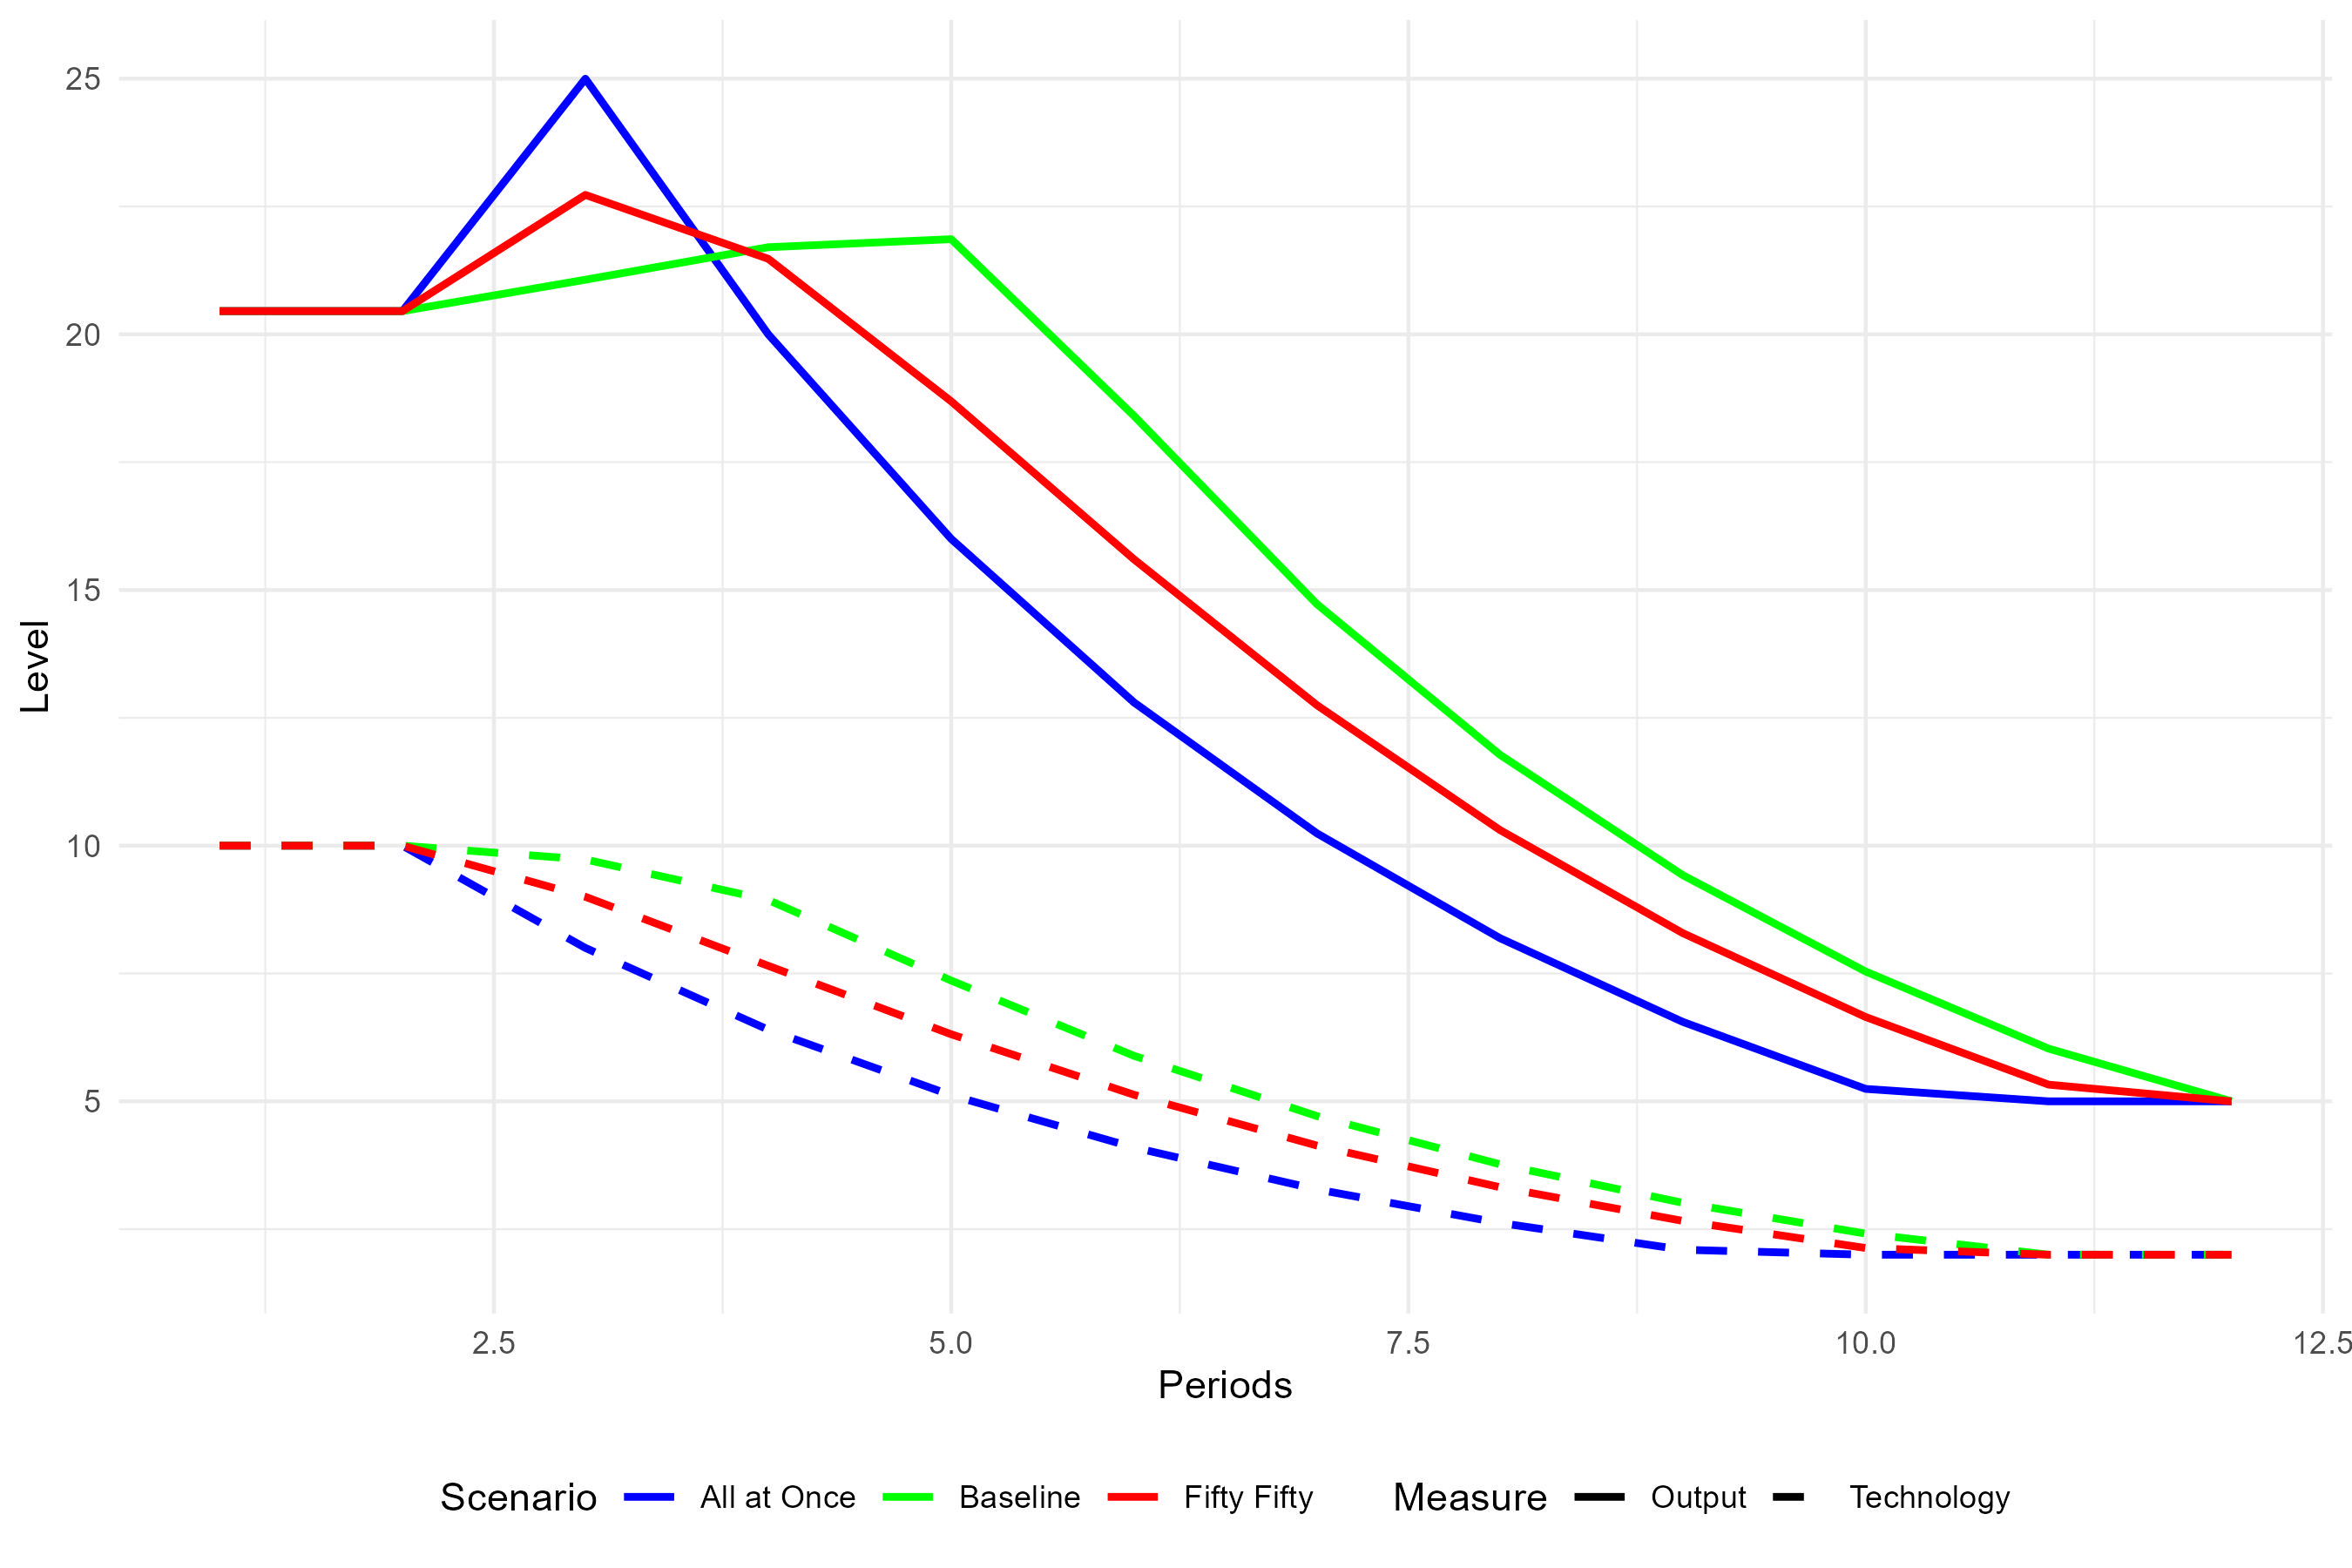
\includegraphics[width=0.9\textwidth]{Output_Tech_Levels.jpg}
    \caption{Output and Technology Time Paths}
    \label{fig:output_and_tech}
\end{figure}

In all cases, populists come to power at date $t=0$ and begin implementing their policies at date $t=1$, moving labor from research into final goods production.  This starts the core mechanism causing an initial boom due to more labor in final goods production and reduces future technology production which eventually dominates and reduces final output.

It is clear that ``all at once" generates the highest but shortest-lived growth rate boom, ``baseline" the lowest but longest-lived growth boom and ``fifty-fifty" something in between.  Technology declines fastest in the first case since 100\% of the labor in research is moved all at once and slowest in the ``baseline" case where labor is moved more slowly.

If political support for the populist government is positively correlated with output - which seems reasonable - then the ``baseline" case also maximizes the populist's time in office.  Continuing with this logic suggests that we should find in the data that larger initial booms are inversely correlated with populist's length of time in office.

While we are using our model for analytical purposes only, not calibrating it to match any specific real world data, we report and explain our key parameter values: $A(0) = 10$, $A_{min}=2$, $L=1$, $\delta_A = 0.2$, $\delta_k = 0.1$, $\theta = 1.1$, $\alpha = 0.5$, and $r^* = .1$. Our results - the basic shapes of the time paths - are very robust to a wide range of parameter values.  

We chose $\alpha = 0.5$ to give equal weight to capital and labor. Lowering $\alpha$ strengthens the effect of our policy by raising the relative importance of labor in final goods production.  We set capital's depreciation rate to 0.1 as in \cite{Mendoza1991} or \cite{UribeSchmitt2017} and simply doubled it for technology's depreciation rate which is 0.2, a little higher than the 0.15 in \cite{DouEtAl2024}.

Finally, we assume a nonzero minimum technology stock, $A_{min}=2$, that is lower than the initial stock $A(0)=10$. While we believe we see technological backsliding as a result of these populist reallocation policies, we find it a bit extreme to imagine that they return all the way to $A=0$.  At the very least, we'd expect the populists either to be removed from power by vote or revolt before that point and, hence, a minimum technology assumption seems reasonable.

\subsection{Monetary Policy and Inflation}

The traditional literature on populist economic policy assumes most of the action comes from overly expansive monetary and fiscal policy, usually in an open economy with a fixed exchange rate regime.  Any real or micro-level policies are seen as generally playing a secondary role (see, \cite{DornbuschEdwards1991}).

We do not dispute that populist governments might employ over-expansive monetary and fiscal policies.  Our contribution, rather, is to give a real-economy basis for the boom-bust cycles and bouts of inflation so often observed in practice. The populist government may also engage in monetary-fiscal overstimulation and that would indeed worsen the inflationary results and may even add to the amplitude of the boom-bust cycle in practice but it is not required in order to generate the basic cycles or inflation itself.

We imagine a populist government following traditional money growth rules based on the quantity equation of money.  This is historically relevant but more importantly is intended to be as neutral as possible a monetary policy in order to emphasize that the results in our model come from the real-sector policy, not monetary policy.  In particular, we assume that policy makers set the growth rate of money equal to the expected growth rate of trend output plus an inflation target, here assumed to be zero. Given constant money velocity, then, $\% \Delta M_t = (\Pi^T =0) + \% \Delta y_t = \%\Delta y_t$.

In our model, real GDP is determined at each date, but its growth rate for the next period is not known and, to be consistent with the timing convention of our model, the stock of money is end-of-period money and requires forecasting growth rates.  Along with all other agents, policy makers expect the relevant growth rates to continue to be whatever the cumulative average growth rate is at that point in time.

While the growth rate of money will be equal to the cumulative average of past GDP growth, inflation will equal the growth rate of the money supply minus the actual growth rate of GDP. In particular, $\Pi_t = \% \Delta M_t - Av(\% \Delta y_t)$. In early years this will mean inflation is under target and in later years, above target, as seen in Figure \ref{fig:Case three output inflation} for case (3), the ``baseline case".

\begin{figure}[t!]
    \centering
    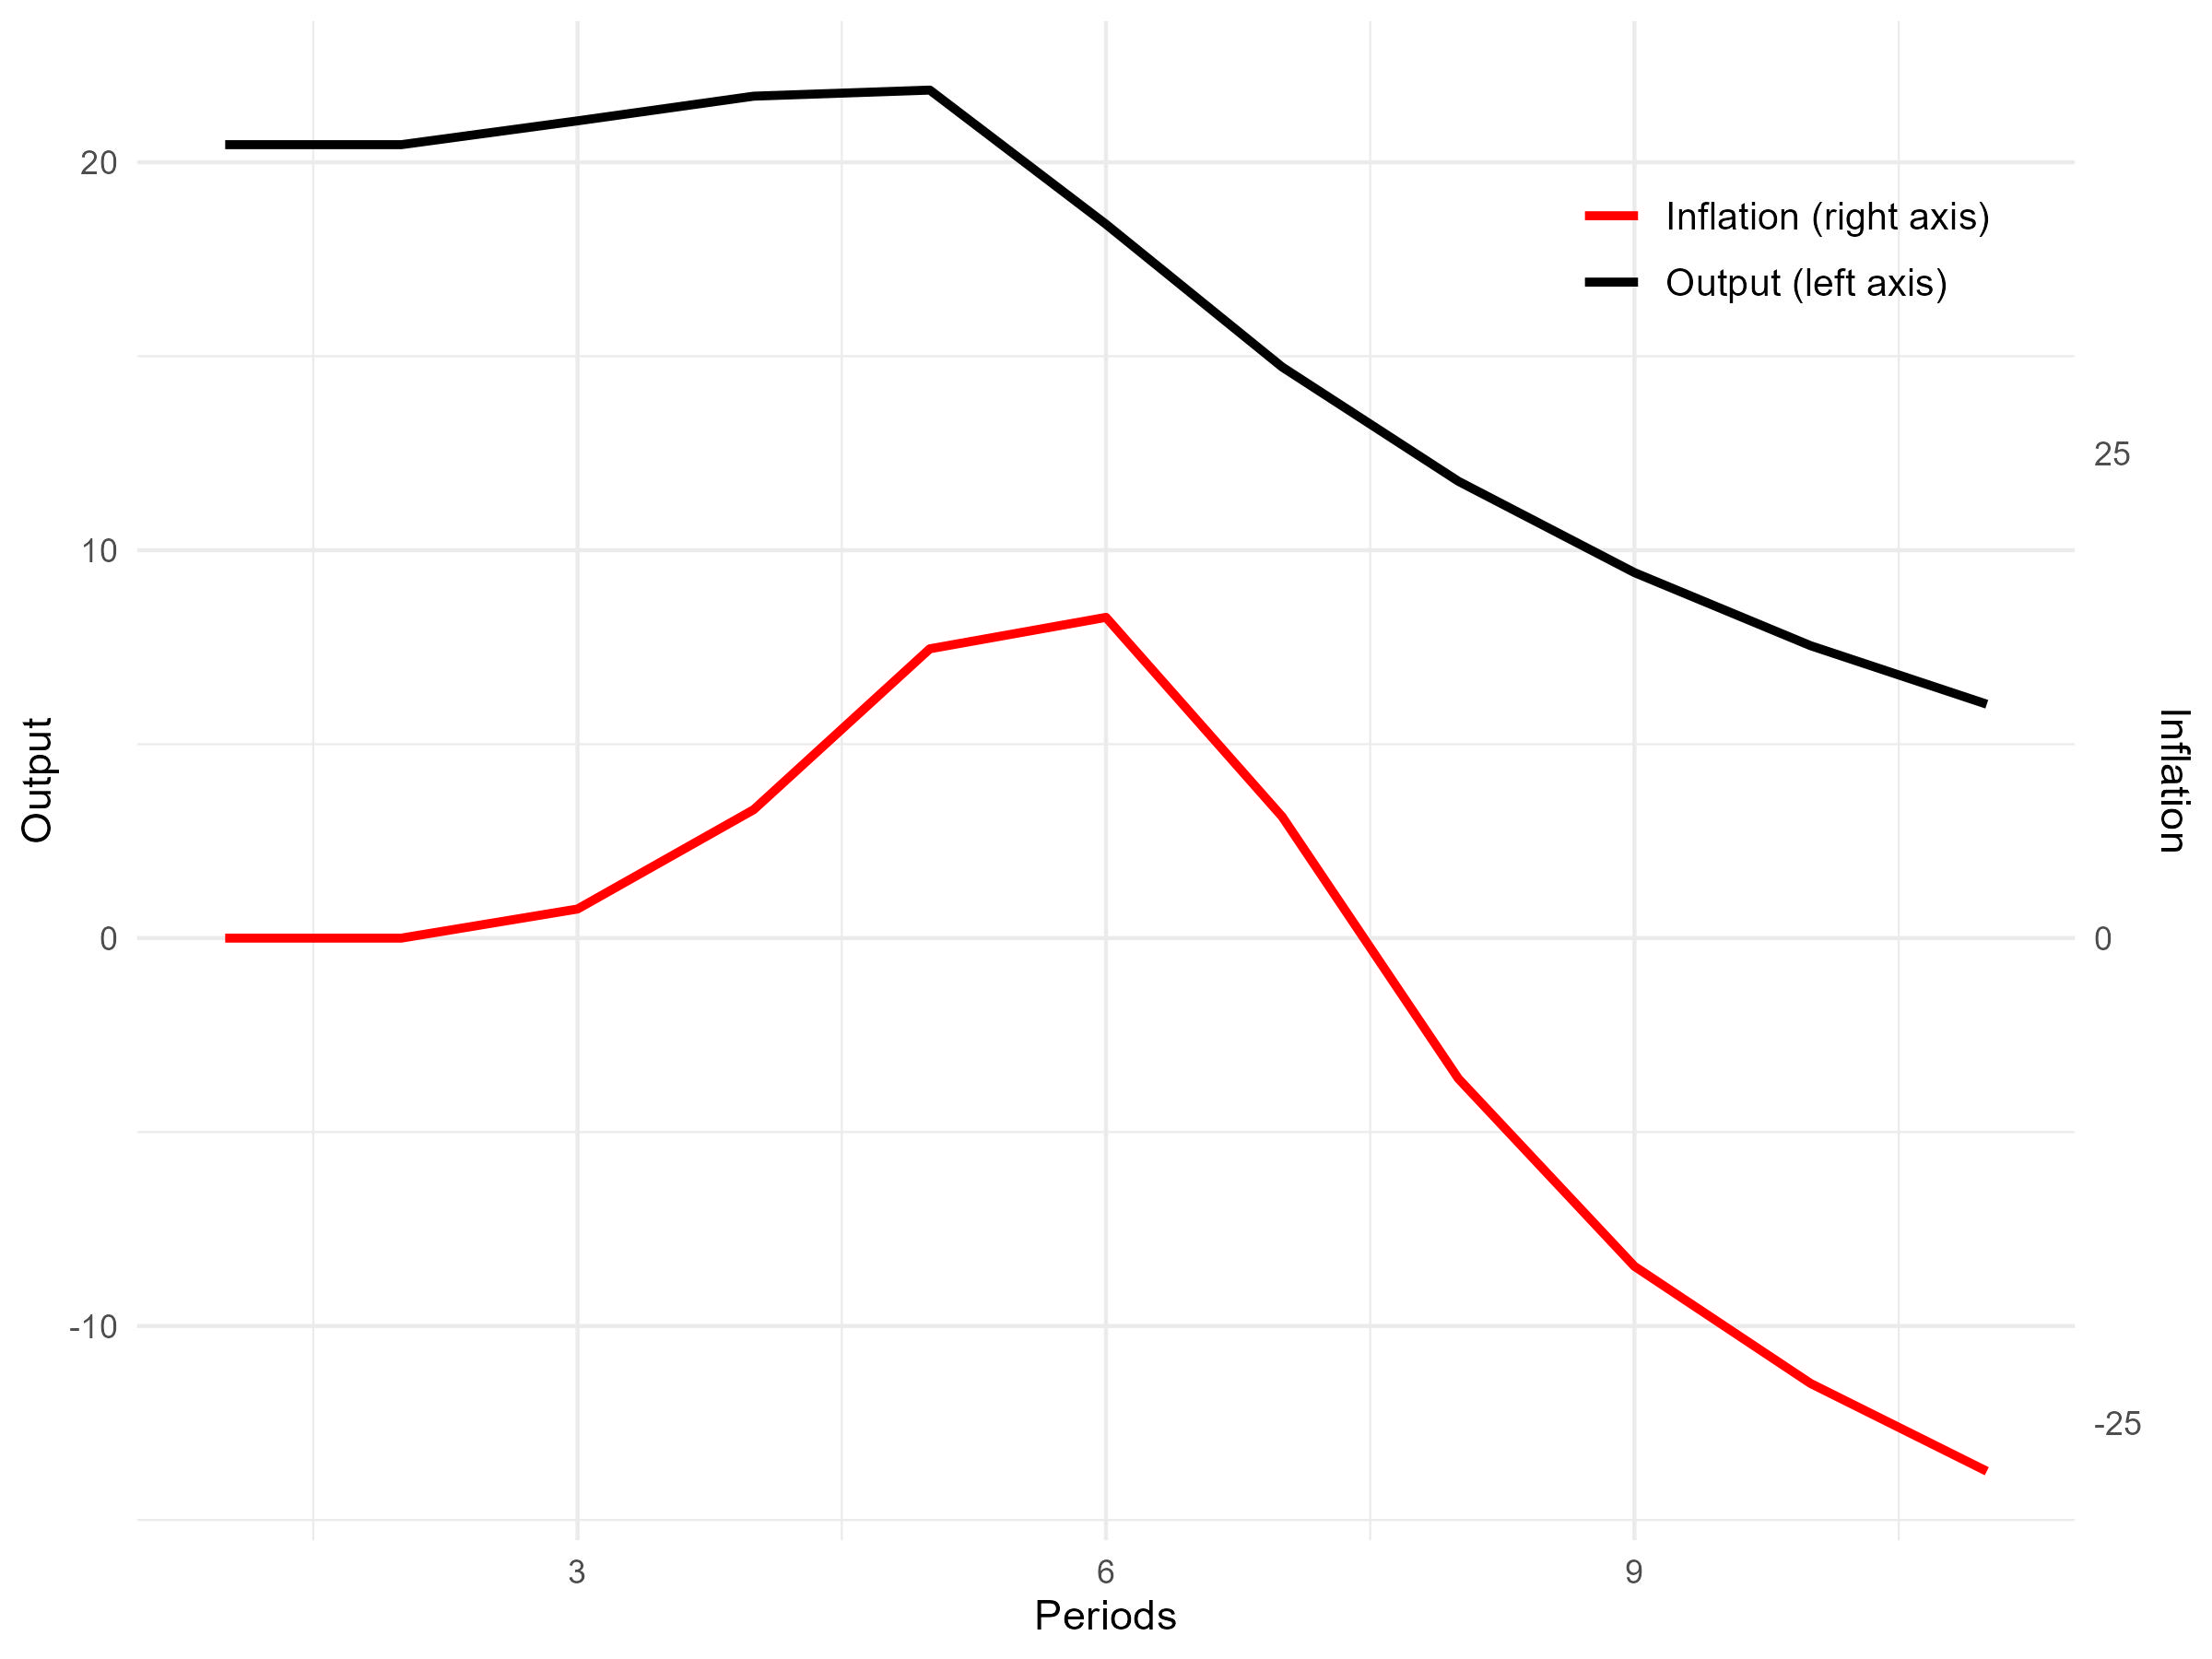
\includegraphics[width=0.9\textwidth]
    {3_Baseline_Output_and_Inflation.jpg}
    \caption{Baseline Case: Inflation and Output}
    \label{fig:Case three output inflation}
\end{figure}

Initially growth expectations, based on the historical data to date (i.e., steady state), sets money growth to zero.  After the populist's re-allocation policy is initiated, expectations are updated to include the past (zero) and current growth (in Figure \ref{fig:Case three output inflation}, 3\%) for an average of 1.5\% expected output growth. In that period, money growth is set equal to expected output growth but output actually grew faster generating mild disinflation.  That pattern continues in the short run, but by the middle run (in Figure \ref{fig:Case three output inflation}, around date 3), the growth rate of output slows but the cumulative probability weight of past growth is strong, so money continues to be printed faster than current output leading to a bout of inflation for several periods that then turns negative as money growth chases collapsing output. Appendix Figure (\ref{fig:Inflation Rates Compared}) presents the paths of inflation for all three example cases.

The price level is found in each period by solving for equilibrium in the real money market: $M_t^s / P_t \equiv m^s_t=m^d_t=c_t(1/i_t +1)$.  Both $M_t$ and $c_t$ are known since money is determined by policy and consumption is constant.  The nominal interest rate is $i_t = r^* + E_t \pi_{t+1}$ which includes expectations of the next period's inflation.  This number is taken as given at the beginning of the period in order to determine household demand for end-of-period real money holdings and therefore cannot include current period inflation as it is not yet determined. Therefore we use the same expectations assumptions as before, averaging past inflation, but excluding the current period's inflation rate. This allows the price level to be uniquely determined at each point in time and allows the nominal interest rate to adjust along with inflation expectations and a constant world real interest rate. The other option here would be to assume that the nominal interest rate is the steady state rate. Doing this makes real money demand constant in this model - a requirement under the perfect foresight assumption since real money balances form a non-stable difference equation - and requires that money changes pass one-for-one to the price level in real time. Doing this generates the same basic path for inflation but shifts it leftward (i.e., bringing the bout of inflation forward in time) and lowers its magnitude slightly so it is essentially tracing the path of the growth rate of money.

Our model suggests that when inflation rises then falls in a populist economy, it is driven more by the real-economic effects and a well-intentioned monetary policy response.  When inflation rises and then continues to rise for a longer-period, it is more likely due to over-stimulative monetary policy.  Hence, we can begin to think about ``real-sector" populists who primarily pursue real sector re-allocation policies in the vein of the one we study versus ``Dornbusch-Edwards" populists who primarily pursue overly expansionary monetary and fiscal policy.  These categories are not mutually exclusive at all. A populist government may certainly pursue them both.  But when there's a difference, our model helps make sense of the difference.

\subsection{The Whole Model}

Figure (\ref{fig:baseline_all_variables}) presents the remaining results for the ``baseline" case. The paths of output, technology and inflation were discussed previously.  The path of consumption is flat, as already explained, in the open economy context with full capital mobility and flexible prices.  This leaves investment and net exports (right-hand side of Figure (\ref{fig:baseline_all_variables})) which are interrelated.  Figures for the all-at-one and fifty-fifty case are in the Appendix.

\begin{figure}[h]
    \centering
    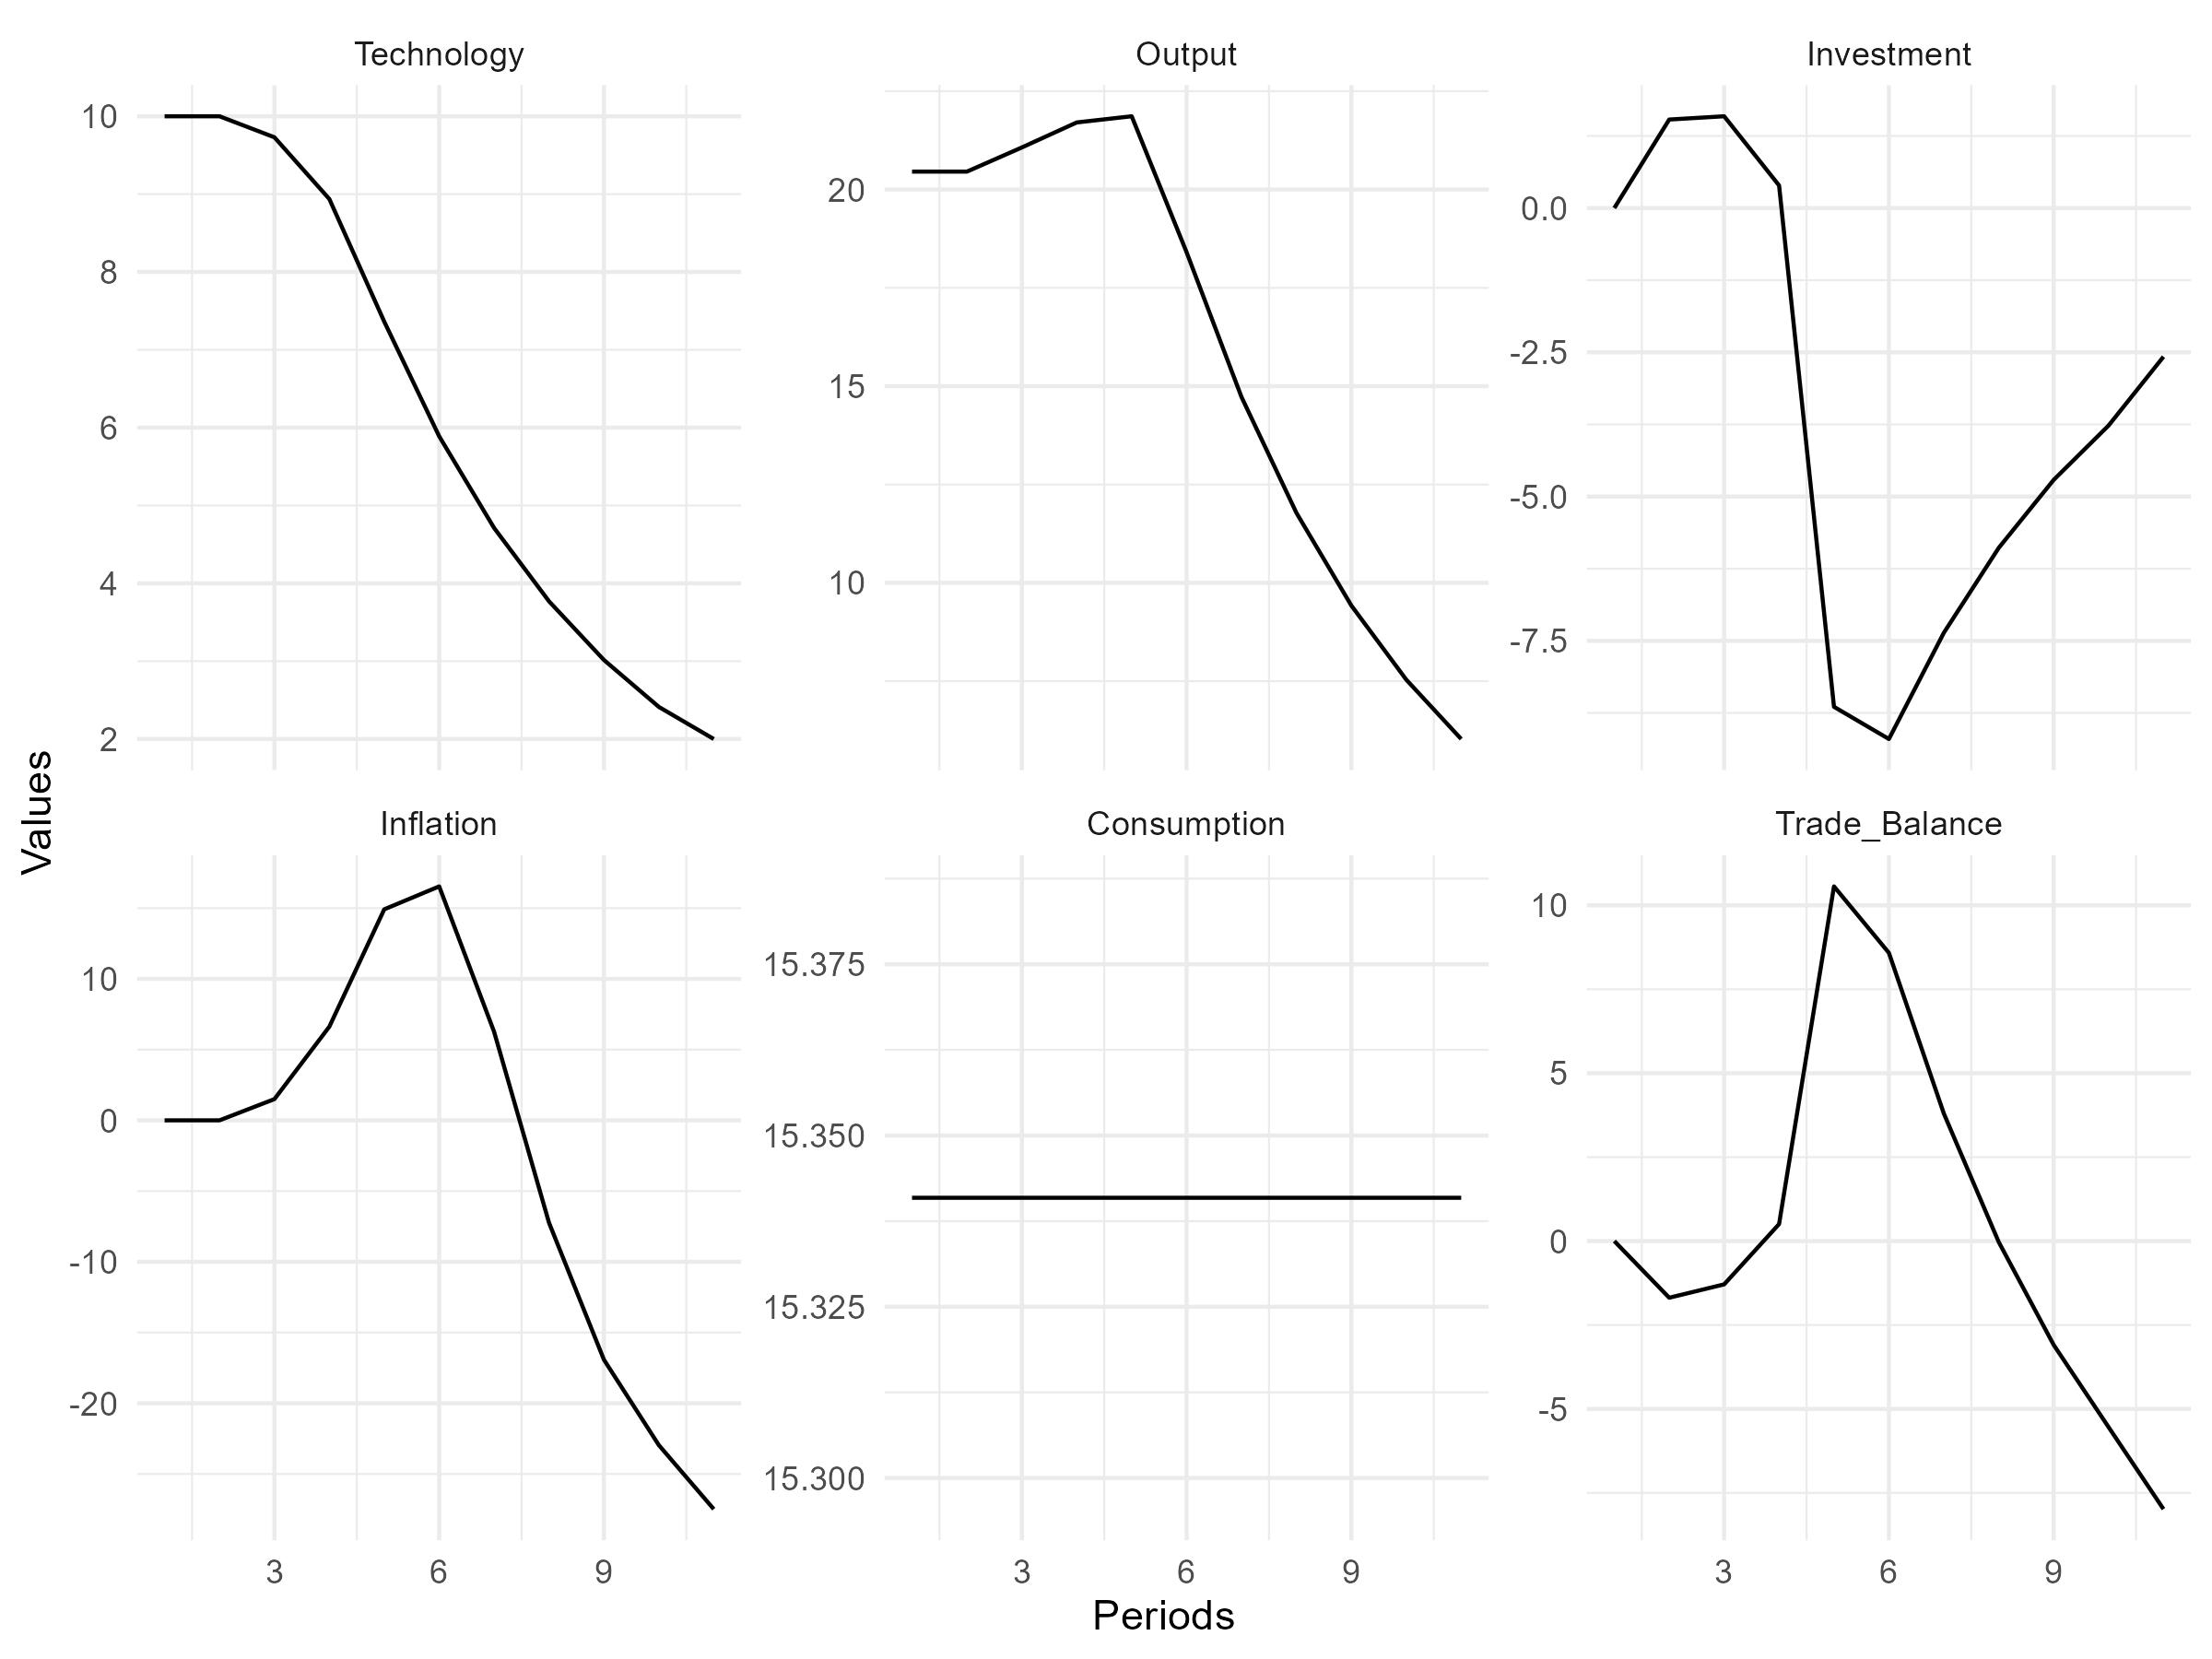
\includegraphics[width=0.9\textwidth]{3_Baseline_Main_Variables.jpg}
    \caption{Baseline Case: Main Variables}
    \label{fig:baseline_all_variables}
\end{figure}

The predictions of the model for the trade balance derive from investment and the net export equation,

$$NX_t=y_t-c_t-\Delta k_t -\delta_K k_{t-1}.$$

Upon impact in the first period, policy makers move ``elite" labor into final goods production which leads to a boom in output while consumption remains unchanged at its steady state level.  Investment today, however, is based on expectations of the marginal productivity of capital in the following period via equation (\ref{MPK=r}), restated here, $\alpha k_{t}^{\alpha-1}A_{t}^{1-\alpha}l_{1,{t+1}}^{1-\alpha} = r^*+ \delta_K$.

The policy we consider is one where policy makers credibly pre-announce the path of labor in both sectors, therefore $l_{1,t+1}$ is known with certainty. It is higher than $l_{1,t}$ initially, raising the next period's marginal productivity of capital.  Initially investment rises faster than output driving a trade deficit during the boom phase.

The trade deficit continues as long as investment is high enough to offset the decline in technology, about 3-4 periods in this scenario.  Thereafter, as investment falls and the capital stock declines toward its new, low-technology steady state, the trade balance turns positive. The paths of investment and the trade balance are not central to our story but there is evidence that many populist economies ran trade deficits during their boom periods. We next take the complete model and focus on the key aspects unique to populism, namely the walking stick pattern and it's cause, and test it.

\section{Empirical Strategy} 
We test the walking stick hypothesis in three stages: First, in order to motivate our core hypothesis, we divide and assign the populist regimes according to their monetary expansion levels in accordance with the respective country’s own median, to capture the differences between Dornbusch-Edwards and real-sector populists. Second, we specify our main empirical model, a dynamic two-way fixed-effects (TWFE) panel regression to test the walking stick pattern in real GDP Growth and its mechanisms. Third, we test the robustness of our findings from the TWFE model through different configurations of this model, as well as with the utilization of a Panel Vector Autoregression (PVAR) and its resulting Impulse Response Functions (IRFs), which is useful in assessing the short-term real economic shocks of a populist regime. We finally present an Error-Correction Model (ECM) with fixed effects, to check if there are deviations from the steady state of real GDP growth in the aftermaths of a populist regime.

\subsection{Stage 1: The data}

Our study covers 62 countries between the years 1970-2019. The data for real GDP, inflation, M2, and total factor productivity (TFP, at current PPPs with USA = 1) come from the Global Macro Database \cite{GMD2025}, Penn World Table \cite{PennWorldTable}, and World Bank \cite{HaEtAl2023}. We build a binary index of populist regimes by combining the lists from \cite{BallFreytag2019} and \cite{FunkeEtAl2023}. \cite{FunkeEtAl2023} provides a robust list based on the consensus of other scholars and other lists.  \cite{BallFreytag2019} provide a deeper look at Latin American countries specifically and essentially add Guatemala and Nicaragua to the Funke et al. (2023) list.\footnote{\cite{BallFreytag2019}, follow older political science literature such as \cite{Weyland2001} to build their database.} Populist regimes, nevertheless, are relatively rare and populist years only constitute approximately 10.05\% of the total 3,720 government-years in our sample. In addition, even though selecting M0 as the monetary policy variable would have made more sense, the data is incomplete for many countries after the monetary union phase of the EU. Thus, such data scarcity problems make some econometric methods more difficult, therefore we opted for an unbalanced panel with M2 as the monetary policy tool. We discuss any relevant issues with scarcity or our econometric approach as they arise in our analysis. 

We draw several distinctions in our data.  We want to distinguish between populists and non-populists, then within populists we want to explore differences between Dornbusch-Edwards and real-sector populists.  Since a key difference is the overly expansive monetary policies in traditional Dornbusch-Edwards populist regimes, our populism index divides cabinets into three groups: Non-populists, Low-M2 populists (those with M2 growth below their own country’s median M2 growth rate ), and High-M2 populists (those with M2 growth above their own country’s median M2 growth rate). Since all the countries in the data set have both populist and non-populist governments, we compare each populist episode to its own institutional framework. If the annual M2 growth is beneath the country's full-sample median, we call it low-M2; if it is above the median, we call it high-M2. This rule naturally distinguishes episodes that appear more like "real-sector" populism from those that are the Dornbusch–Edwards monetary-expansion type. Thus, Table (\ref{tab:gdp_infl_tfp_m2}) shows the results for each group's performance regarding annual real GDP growth, CPI inflation, and TFP. For each cabinet term, we report: first the percentage of years with positive growth then the relative peak and relative trough, which are calculated by taking the term's highest and lowest points and calculating the difference between those extreme years to the country's long-term median. We do the same for inflation and TFP. 

\begin{table}[htbp]
\caption{GDP, Inflation \& TFP dynamics by M2-growth intensity}
\label{tab:gdp_infl_tfp_m2}
\resizebox{\textwidth}{!}{%
\begin{tabular}{lcccc}
\hline
\textbf{Statistic} & \textbf{Non-populists} &\textbf{All Populists} & \textbf{Populists Low-M2} & \textbf{Populists High-M2} \\
\hline
Avg. Time in Office      & 3.91  & 4.55  & 3.79*  & 5.20*      \\
Share \%$\Delta y > 0$    & 84.98 & 81.06 & 86.63* & 76.33*    \\
Rel-Peak \%$\Delta y$     & 1.19*  & 2.27*  & 1.03* & 3.31*    \\
Rel-Trough \%$\Delta y$   & -2.44* & -4.06* & -2.46* & -5.41*  \\
Share \%$\Delta \pi > 0$  & 48.04 & 49.00  & 40.25* & 56.42*  \\
Rel-Peak \%$\Delta \pi$   & 6.76  & 1210.79  & 1.09  & 2236.40  \\
Rel-Trough \%$\Delta \pi$ & -10.09* & -972.39* & -2.18* & -1794.97* \\
Corr Time in Office \& Rel-Peak \%$\Delta y$ & 0.31 & 0.52 & 0.50 & 0.49 \\
\hline
\end{tabular}%
}
\end{table}

Our hypothesis is based on the theoretical model and is thus straightforward: real-sector populism (Low-M2 populists) should cause a boom in output, subsequently met with a longer bust, mild inflation, and a gradual fall in TFP. Dornbusch–Edwards populism (High-M2 populists) depends more on increasing the money supply. This means that output will still be low, but inflation will be higher and last longer. TFP does not necessarily have to go down.

\begin{table}
\caption{Share of years with positive TFP growth}
\label{tab:tfp_growth_years}
\resizebox{\textwidth}{!}{%
\begin{tabular}{lcccc}
\hline
\textbf{Statistic} & \textbf{Non-populists} & \textbf{All Populists} & \textbf{Populists Low-M2} & \textbf{Populists High-M2} \\
\hline
Share \%$\Delta$TFP $>0$ & 51.85 & 46.07 & 39.89$^{*}$ & 52.52$^{*}$ \\
\hline
\end{tabular}%
}
\begin{tablenotes}
$^{*}$ indicates statistical significance at the 10\% level. 62 countries.
\end{tablenotes}
\end{table}

Table (\ref{tab:tfp_growth_years}) suggests that Non-populists and Low-M2 populists have similar terms and lengths of growth (about 85–86\% of cabinet-years with $\Delta y > 0$), with small peaks and troughs (about 1.0–1.2\% and −2.4\%). It is indeed interesting that Low-M2 populists have less inflation than Non-populists (peak $\approx 1.09\%$; trough $\approx −2.18\%$). In comparison, High-M2 populists have shorter booms (about 76\% of the time have $\Delta y > 0$), but sharper peaks ($\approx 3.31\%$) and deeper troughs ($\approx −5.41\%$), as well as very high inflation, which aligns with \cite{DornbuschEdwards1990} , as well as \cite{BallFreytag2019}. However, it is the TFP that differentiates the two types of populists: Low-M2 populist governments, which mimic our real-sector populists, have the shortest TFP growth periods with $\Delta TFP > 0$ in roughly 40\% of years. For High-M2 populists, this number is about 52\%. 

To make sure that the differences we see are not just noise from the samples, we also conduct Welch two-sample t-tests\footnote{Full results, including p-values, available upon request}  on cabinet-level outcomes to determine if the means differ between our contrasting groups: first, Non-populists versus All Populists, and second, Low-M2 versus High-M2 populists, explicitly accounting for unequal variances and sample sizes. Results are significant at $p < 0.10$. The tests confirm that the differences are mostly in boom–bust magnitude and inflation drift (more pronounced under High-M2). For TFP, the main difference is that High-M2 $>$ Low-M2 in the share of positive-TFP years, and Non-populists vs All Populists is not significantly different.

We can deduce from the initial results that populist and non-populist governments show different macro patterns, and the distinction of two groups within populism is important: Low-M2 cases exhibit prolonged economic booms accompanied by moderate inflation and a relatively short-lived (TFP) growth, indicative of misallocation. In contrast, High-M2 cases are characterized by shorter but stronger booms and significant inflation without a systematic decline in TFP, hinting at a monetary expansion. We now formally test these differences in a TWFE framework that controls for country and year effects and calculates the distinct impacts of Low-M2 and High-M2 regimes on growth, inflation, and TFP.

\subsection{Stage 2: Two-Way Fixed Effects Model}
We employ a Dynamic Two-Way Fixed Effects Model (TWFE) model to trace the dynamic trajectory of economic outcomes in the years following a populist’s entry into power while also controlling for time-invariant country (e.g., institutions) and year (e.g., a global recession) characteristics. We implement this strategy within the frame of Low-M2 and High-M2 Populists. The model is in the following form:

\begin{multline}
    Y_{it}=\alpha_i+\gamma_t+\sum_{j \in \{Low M2, High M2\}}\beta_{1j}\left(P^{j}_{it} \times T_{it} \right) \\
    + \sum_{j \in \{Low M2, High M2\}}\beta_{2j}\left(P^{j}_{it} \times T^{2}_{it} \right)+\delta_1T_{it}+\delta_2T^{2}_{it}
    \label{TWFE_equation}
\end{multline}

Where $Y_{it}$ is the rGDP in country $i$ at year $t$. $P^j_{it}$ is an indicator variable for populist type $j$ (Low-or-High M2), and $T_{it}$ is the time in office for the government in question. The interaction between the populist indicators and the quadratic in time allows for the estimation of a unique dynamic path for each populist group, relative to the baseline, which is the non-populist governments. Thus, we expect a walking stick pattern for a group $j$ of the populists, which means a statistically significant value for $B1_j$ and a negative for $B2_j$.

Table (\ref{tab:twfe_gdp_tfp}) presents our regression results. The first column presents the results of GDP growth as the dependent variable and the second column of TFP growth as the dependent variable in equation (\ref{TWFE_equation}).  

\begin{table}[ht]
\centering
\caption{TWFE Walking Stick Effects on GDP and TFP Growth}
\label{tab:twfe_gdp_tfp}
\resizebox{.8\linewidth}{!}{%
\begin{tabular}{lcc}
\hline
\textbf{Variable} & \textbf{GDP} & \textbf{TFP} \\
\hline
groupPopulist (Low M2) & -0.229 & 0.193 \\
                       & (0.547) & (0.767) \\
groupPopulist (High M2) & -0.237 & 1.294 \\
                        & (0.633) & (0.909) \\
Years in Office & 0.082$^*$ & 0.035 \\
                & (0.043) & (0.038) \\
(Years in Office)$^{2}$ & -0.002 & 0.000 \\
                        & (0.001) & (0.001) \\
groupPopulist (Low M2):Years in Office & 0.731$^{***}$ & 0.762$^{***}$ \\
                                        & (0.260) & (0.249) \\
groupPopulist (High M2):Years in Office & 0.396 & 0.014 \\
                                         & (0.330) & (0.379) \\
groupPopulist (Low M2):(Years in Office)$^{2}$ & -0.087$^{***}$ & -0.074$^{***}$ \\
                                               & (0.026) & (0.021) \\
groupPopulist (High M2):(Years in Office)$^{2}$ & -0.31 & -0.002 \\
                                                & (0.040) & (0.047) \\
\hline
Num.Obs. & 3534 & 3316 \\
R2       & 0.007 & 0.002 \\
\hline
\end{tabular}%
}

\begin{tablenotes}Standard errors clustered by country. 
GDP and TFP columns report coefficients for GDP growth (\%) and TFP growth (\%), respectively. 
$^{*} p<0.10$, $^{**} p<0.05$, $^{***} p<0.01$.
\end{tablenotes}

\end{table}

The results on GDP growth support our central hypothesis that populists tend to generate walking stick patterns in GDP.  The interaction between the Low-M2 indicator and \textit{Years in Office} is positive and highly significant ($B=0.731$, $p < 0.01$), while the interaction with (\textit{Years in Office}) squared is negative and highly significant ($B=-0.087$, $p < 0.01$), which is a robust evidence of a boom-bust cycle. However, the coefficients of High-M2 Populists are statistically insignificant, stating that their real GDP growth trajectory is not different from the non-populist baseline after controlling for country and year fixed effects. 

To identify real-sector populists we test for our full theoretical mechanism by estimating the model with TFP growth as the dependent variable; results in the TFP column of Table (\ref{tab:twfe_gdp_tfp}).  The results again support our hypothesis. There is a walking stick in TFP growth performance of Low-M2 Populists, as the interaction coefficients are statistically significant both for the linear ($B=0.762$, $p < 0.01$) and quadratic ($B=-0.074$, $p < 0.01$). The data supports the view that real-sector allocation policy causes disruptions that are characterized with an initial boom in productivity and real GDP. However, the erosion of the capacity to innovate, as suggested by our theoretical model, leads to an inevitable bust. In contrast, the results for High-M2 Populists are once again insignificant and not different from the baseline.

\subsection{Stage 3: Robustness Checks }

Before moving on to the complementary evidence from our PVAR model, we implemented five different robustness checks to our TWFE model to assure that our walking sticks are robust. First, we excluded all governments that have a time in office lower than 3 years to rule out bias from interim governments and crises. This does render both real GDP and TFP insignificant.  Given the rarity of populist governments in the data, once we remove the shortest-lived populist regimes there are too few remaining regimes to generate significant results.  Second, we tried a different measure from World Bank for TFP (at constant national prices with 2017 = 1 for each country), which is a delicate variable, but the results have not changed with respect to direction of the effects and the level of significance. Third, to assure that there are not any pre-existing trends, we used leads of our treatment indicator and found no evidence of any pre-existing trend, whereas the TFP coefficients turn insignificant. Fourth, to accommodate possible serial and cross-sectional dependencies, we employed \cite{DriscollKraay1998} adjustments to reconstruct our standard errors. Although there was an increase in standard errors, the primary effects of Low-M2 remained highly significant at conventional levels for both models.

\subsection{Panel Vector Autoregression (PVAR)}

Next, we employ a PVAR model since our inquiry is inherently dynamic and endogenous: upon the ascendance of a populist government, real activity, productivity, and prices exhibit synchronized movements, which subsequently influence political dynamics. A PVAR enables us to model the joint dynamics across multiple countries first, then eliminate time-invariant country heterogeneity through the within demeaning, and finally identify the causal timing of a ``populist entry” on macroeconomic outcomes without imposing single-equation constraints.

Formally, for country $i$ and year $t$, we order the variables as follows,

\begin{equation}
x_{it} = 
\begin{bmatrix}
\text{PopEntry}_{it} \\
\text{TFP}_{it} \\
\text{GDP}_{it} \\
\pi_{it}
\end{bmatrix}
\end{equation}

and we estimate:

\begin{equation}
x_{it} = A_{1} x_{i,t-1} + \cdots + A_{p} x_{i,t-p} + \mu_{i} + \varepsilon_{it}, 
\qquad \varepsilon_{it} \sim \mathcal{N}(0, \Sigma)
\end{equation}

where the subscript $g$ denotes year-over-year growth; $\pi_{it}$ is CPI inflation; and  $\text{PopEntry}_{it}$ is a binary indicator equal to one in the first year of a new populist cabinet (zero otherwise). $A_l$ where $l=1,…,p$ are 4×4 coefficient matrices, $p$ is the lag length chosen by information criteria, $\mu_i$ are country fixed effects removed by the within transform, and $\varepsilon_{it} $ are reduced-form innovations with covariance $\Sigma $. For the IRFs we orthogonalize shocks via the Cholesky factorization $\Sigma =PP′$ with PopEntry ordered first, and trace responses to a one-standard-deviation structural innovation in PopEntry.

To prevent sample loss due to lack of M2 in dynamic estimations, our core model employs four variables—PopEntry, TFP growth, real GDP growth, and inflation—and we present $p=5$ lags, selected from 1–5 based on standard information criteria. Nevertheless, we still lose the sample of 6 countries of our dataset, namely Bulgaria, Czech Republic, Croatia, Estonia, Latvia, Lithuania, and Slovakia. The Im-Pesaran-Shin Test \cite{ImEtAl2003} is used to check for stationarity in growth/inflation series. The estimation stacks the demeaned panels and fits a pooled VAR without a constant (the constant is added as a robustness check). Impulse responses show how a shock to PopEntry that is one standard deviation away from the mean affects it over a period of 20 years. The uncertainty is based on a vector-residual bootstrap with $B=2000$. The graphs on figures show the point estimate and the $\pm1$-SE guides. We also calculate 68/95\% percentile bands.

\begin{figure}[!ht]
    \centering
    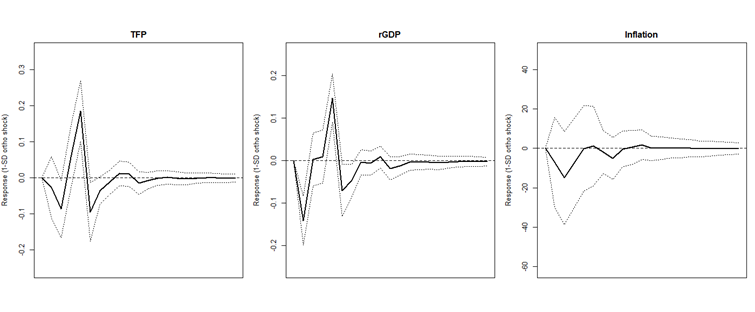
\includegraphics[width=\textwidth]{IRF_non_pop.png}
    \caption{IRFs: Non-Populists}
    \label{fig:IRF_non_pop}
\end{figure}

\begin{figure}[!ht]
    \centering
    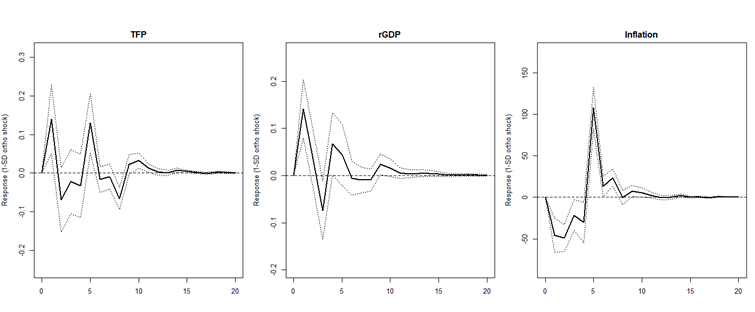
\includegraphics[width=\textwidth]{IRF_all_pop.png}
    \caption{IRFs: All Populists}
    \label{fig:IRF_all_pop}
\end{figure}

According to Figure (\ref{fig:IRF_non_pop}), there isn't an inflation spike, and TFP and GDP show J-Curves, indicating that non-populists have a medium- or long-term focus. In contrast, Figure (\ref{fig:IRF_all_pop}) show the classic boom-then-bust pattern for All-Populists: a sharp rise in real GDP growth followed by a drop in growth in the middle of the horizon, with short-lived TFP spurts and a spike in inflation. That difference is exactly what we mean by ``walking-stick": an early surge that later strikes downward against real performance. This only happens when the entry is populist.

\begin{figure}[!ht]
    \centering
    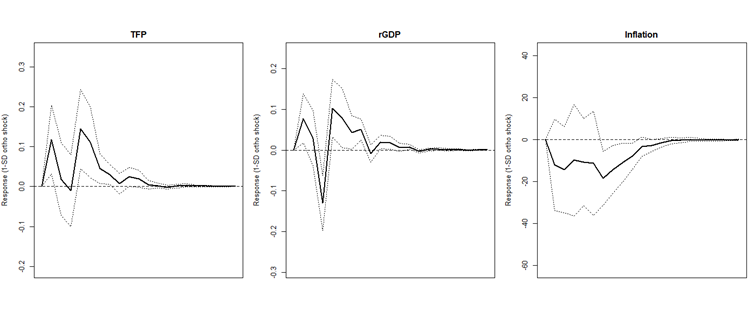
\includegraphics[width=\textwidth]{IRF_low_m2_pop.png}
    \caption{IRFs: Low-M2 Populists}
    \label{fig: IRF_low_m2_pop}
\end{figure}

When we examine Figure (\ref{fig: IRF_low_m2_pop}) to analyze our core point of interest, the Low-M2 populists, we see a walking stick on the real side. Following the initial bump at after the entry, real GDP growth slows down at about three to five years before returning to the growth zone again, while inflation falls and stays small. TFP growth has a small, statistically significant bump at the beginning that goes away. This is precisely what a strategy for the real sector would look like if the money supply were to be limited by politicians, in order to gradually maximize their stay in office as hypothesized and shown in the simulations part. Policies that ``punish elites" and shift protection and budget priorities toward commodities and manufacturing cause a short disruption as laborers and executives are moved around. We are still cautious because the TFP rise is only temporary and close to zero in the bands.

\begin{figure}[!ht]
    \centering
    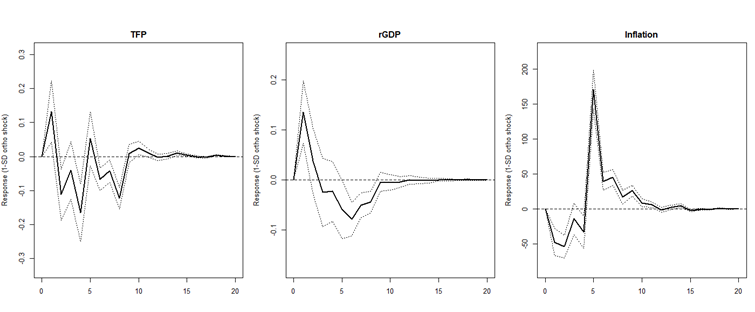
\includegraphics[width=\textwidth]{IRF_high_m2_pop.png}
    \caption{IRFs: High-M2 Populists}
    \label{fig:IRF_high_m2_pop}
\end{figure}

Regarding the High-M2 populists, Figure (\ref{fig:IRF_high_m2_pop}) shows that the mechanism is based on demand and money. After a short-term rise, there is a big jump in inflation about three to six years after entry. GDP growth crashes down at medium-term horizons, and TFP does not show any lasting improvement. Inflationary monetary policy and distorted price signals diminish real gains and discourage investment, resulting in the prolonged return expected by the walking-stick hypothesis.

\subsection{Error Correction Model}

We finally utilize an error-correction model (ECM) to capture  both the long-run relationship and the short-run adjustments effectively in the case where rGDP and TFP are cointegrated. Our specific inquiry examines whether the emergence of a Low-M2 populist regime alters rGDP's trajectory to a long-run path lower than the pre-regime equilibrium path. We conduct unit-root tests with Fisher-ADF \cite{MaddalaWu1999}, Choi-Z \cite{Choi2001}, and Hadri \cite{Hadri2000} frameworks (including fallbacks). In all cases, two of the three or all three reject unit-roots.  We established panel cointegration between $log(rGDP)$ and $log(TFP)$ through a bootstrap Westerlund test optimized for unbalanced panels (see \cite{Westerlund2007} and \cite{PersynWesterlund2008}) and subsequently estimated a two-way fixed-effects ECM for $\Delta log rGDP$.  The error correction term (ECT) is derived from a country-FE long-run relationship incorporating Low-M2 interactions. As expected, the bootstrap Westerlund test confirms that there is cointegration between the two variables.

The model consists first of a regime-aware long-run ECM,

\begin{equation}
    y_{i,t}=\alpha_i + \beta x_{i,t} + \theta R_{i,t} + \kappa \left( R_{i,t} \cdot x_{i,t} \right) + u_{i,t},
    \label{eqn:regime-aware_long-run_ECM}
\end{equation}

an Error Correction Term (ECT) defined as

\begin{equation}
    ECT_{i,t-1} = y_{i,t-1} - \left[ \alpha_i + \beta x_{i,t-1} + \theta R_{i,t-1} + \kappa \left( R_{i,t-1} \cdot x_{i,t-1} \right) \right],
    \label{eqn:ECT}
\end{equation}

and, finally, the regime-aware short-run FECM with speed shift,

\begin{equation}
    \Delta y_{i,t} = \left(\phi_0 - \phi_1 R_{i,t} \right)ECT_{i,t-1} + \gamma \Delta y_{i,t-1} + \delta_0 \Delta x_{i,t} +  \delta_1 \Delta x_{i,t-1} + \lambda_i + \tau_i + \varepsilon_i,
    \label{eqn:FECM}
\end{equation}

where $y_{it}$ denotes log(realGDP), $x_{it}$ log(TFP) and $R_{i,t}$ the regime dummy (either Low-M2 populist or High-M2 populist). Equation (\ref{eqn:regime-aware_long-run_ECM}) is estimated in levels with country fixed effects $\alpha_i$; its fitted part at $t-1$ yields $ECT_{i,t-1}$ using $x_{i,t-1}$ and $R_{i,t-1}$. 

Equation (\ref{eqn:ECT}) is then estimated for $\Delta y_{i,t}$ with one lag of $\Delta y$ and $\Delta x$, a current-period $\Delta x$, country and year fixed effects ($\lambda_i$ and $\tau_i$, respectively) , and country-clustered standard errors. Hence, we pay attention to the regime parameters $\theta$, reflecting any long-term shift in the $y–x$ relationship, and $\kappa$, indicating a shift in its slope. The short-term adjustment is examined separately through the ECT×Regime term.

\begin{table}[htbp]
\centering
\caption{ECM coefficients: Populist level and TFP interaction by M2-growth regime}
\label{tab:ecm_lr_results}
\resizebox{\textwidth}{!}{%
\begin{tabular}{lcccc}
\hline
 & \multicolumn{2}{c}{\textbf{High M2-Growth}} & \multicolumn{2}{c}{\textbf{Low M2-Growth}} \\
\textbf{Parameter} & \textbf{Estimate (SE)} & \textbf{p-value} & \textbf{Estimate (SE)} & \textbf{p-value} \\
\hline
Populist level shift ($\theta$) &
$-0.348$ (0.239) & 0.145 &
$0.329$ (0.277) & 0.234 \\[3pt]
TFP interaction ($\kappa$) &
$-0.886^{***}$ (0.318) & 0.005 &
$-0.817^{***}$ (0.410) & 0.046 \\[3pt]
Short-term adj. ($\phi_1$) &
0.005 (0.005) & 0.364 &
0.004 (0.004) & 0.353 \\[2pt]
\hline
\end{tabular}
}
\begin{tablenotes} Long-run (equilibrium) coefficients from an Error Correction Model. 
$\theta$ measures the level shift under populist regimes; 
$\kappa$ captures the change in long-run elasticity with respect to TFP. 
Standard errors are heteroskedasticity-robust and clustered by country.
$^{*} p<0.10$, $^{**} p<0.05$, $^{***} p<0.01$.
\end{tablenotes}

\end{table}

The long-run Error Correction Model (ECM) estimates in Table (\ref{tab:ecm_lr_results}) indicate that, when Low-M2 (real sector) populists take office, the rGDP-TFP slope flattens by around 0.82 ($p < 0.05$) suggesting the economy settles at a lower long-run level of rGDP for the same TFP. The insignificant $\theta$ means that Low-M2 populists don’t start from a higher or lower income level.  The difference comes only from how weakly measured TFP is reflected in output. We interpret this as evidence that the productivity channel of Real Sector Populists is weaker. On the other hand, High-M2 populists exhibit an even lower long-run level of rGDP for the same TFP, as seen in the flattening of the slope by about 0.89 ($p < 0.001$). The insignificant $\phi_1$ suggests that both Low-M2 and High-M2 populist regimes appear to be slowing down as GDP gets back to its long-term path. However, the difference isn't sufficient statistically to conclude that their adjustment speed actually changes. As with its Low-M2 counterpart, there is not an extra short-term drop in real GDP growth for High-M2 populists. Even though the boom-bust pattern identified earlier is not part of the ECM story, the long-run deterioration in how productivity translates into growth proves to be common across most of our empirical findings.  

We do not overemphasize our empirical results for TFP and rather suggest future research could focus on specific country cases where TFP can be measured in multiple ways to explore the deeper walking theory implications.  The problem is that TFP is a very elusive variable and acknowledged to be poorly-measured in general.  As Zvi Griliches, one of the pioneers himself explained, "[a]ll the pioneers of this subject [measuring TFP] were quite clear about the tenuousness of such calculations and that it may be misleading to identify the results as ``pure" measures of technical progress" \cite[p.1328]{Griliches1996}.  Therefore we consider our TFP results interesting and when complemented with the path of rGDP largely in line with our theory.  Nevertheless, we do not consider them perfect measures of the theoretical concept of TFP, “A”, in our theoretical model.”

In connection with our PVAR model as well, this can be considered as another example of the “walking-stick” story: policies that put current production first may increase activity in the short-run but they also hurt innovation which brings the economy back to a lower equilibrium. The results show that the error correction term (ECT) is negative and statistically significant, which means that the equilibrium follows a TFP-anchored path. It is indeed interesting, that both Low-M2 and High-M2 populism moves the economy to a lower long-run rGDP equilibrium, with the latter causing a bigger deterioration. This is in line with a productivity-channel interpretation of the “walking-stick” pattern for Real Policy Populists, however, when that same “real” stance is paired with loose money of the Dornbusch-Edwards explanation, cheap credit can keep the inefficient firms not only alive but also scale them up, thus making the TFP mechanism deteriorate further. 

Ultimately, our findings indicate that regimes implementing the populist ideology of “us versus them” in policies seems to create a short-term boom in output leading to a walking stick pattern due to a strong bust with decreasing TFP growth. Adding expansionary monetary policy seems to worsen the scenario highlighting that there seem to be Dornbusch-Edwards populists although distinguishing regimes as purely Dornbusch-Edwards or real-policy is hard. This is not entirely surprising since they are not mutually exclusive categories.  Certainly many regimes engage in real policies and expansionary monetary policy.  Nevertheless, recognizing that these are two different policies and understanding how they interact is valuable in better understanding populist regimes and their economic implications.

\section{Conclusion}

While the economic consequences of populist policies are well documented and seem obvious, neither the exact path of these effects nor theoretical foundations have been assessed thoroughly in the literature. This lack of understanding may also lead to incomplete policy action to prevent populist governments in democratic elections. In an attempt to fill this gap, we add a deeper theoretical backing to analyzing populist macroeconomic policies and results as well as shed new light on the data.  In particular we show that there are policies that should be largely unique to populists - namely, harming elites in the populist's us-versus-them worldview - and these populist policies have severe real effects that generate the boom bust cycles observed historically. The inflation we observe historically may very well have resulted from populist governments ignoring intertemporal constraints and trying to stimulate the economy with aggressive monetary policy, but explaining it no longer requires this assumption. 

However, two observations show that this explanation is not unique. First, non-populist governments also regularly ignored budget constraints and thus created boom bust cycles; this case is not in our interest. Second, we show that populist governments can maintain a reasonable monetary policy. Then other, real and populist-specific policies led to real economic problems that, when combined with reasonable monetary policy, led to high inflation problems.  

We call them walking sticks in reference to the same pattern but focus on the path of real output and inflation and the real policy changes that can cause them. Our model gives a reason why populist policies \textit{per se} generate a walking stick, holding fiscal-monetary policy constant which here means they are conducted reasonably and in good faith. It links the boom-bust or walking-stick results to the populist ideology and resultant policies themselves and thereby uses a widely accepted – ideational – definition of populism, which avoid circular conclusions. Our paper is therefore a first attempt at a theoretical model that organized the historical data in a way which can allow some differentiation between simply bad monetary policy and bad policy ideas, here specific to populists.  Future research can move toward more sophisticated measures of populists and/or complicated models that allow more subtle policies or policy combinations as well as alternative monetary arrangements.




\appendix

\section{Mathematical Appendix}

Households maximize lifetime utility, equation (\ref{utility}), subject to the real, flow budget constraint, equation (\ref{real budget}), and technology's equation of motion, equation (\ref{tech accum}).  Doing so generates the following optimality conditions where $\lambda_t$ is the Lagrangian multiplier on the budget constraint, equation (\ref{real budget}) and $\mu_t$ is the multiplier on the technology accumulation equation (\ref{tech accum}).

\begin{equation}
    \label{L_c}
    \beta^t u_{c_t}=\lambda_t
\end{equation}

\begin{equation}
    \label{L_L2}
    \lambda_t (1-\alpha)k_{t-1}^{\alpha} A_{t-1}^{1-\alpha}(L-l_{2,t})^{-\alpha}(-1)+\mu_t \theta A_{t-1} = 0
\end{equation}

\begin{equation}
    \label{L_k}
    -\lambda_t + E_t \lambda_{t+1} (\alpha k_{t}^{\alpha-1}A_{t}^{1-\alpha}(L-l_{2,{t+1}})^{1-\alpha} +(1-\delta_K)) = 0
\end{equation}

\begin{equation}
    \label{L_A}
    -\mu_t + E_t \mu_{t+1} [\theta l_{2,t+1} +(1- \delta_A )]+E_t \lambda_{t+1}[(1-\alpha) k_t^{\alpha}A_t^{-\alpha}(L-l_{2_{t+1}})^{1-\alpha}]=0
\end{equation}

\begin{equation}
    \label{L_b}
    -\lambda_t + E_t \lambda_{t+1} (1+r^*) = 0
\end{equation}

\begin{equation}
    \label{L_m}
    \beta^t u_{m_t} - \lambda_t +E_t \lambda_{t+1} \left[\frac{1}{1+\pi_{t+1}}\right] = 0
\end{equation}

where $u_{c_t} = {1}/{c_t}$ and $u_{m_t} = {1}/{m_t}$.  In addition to the above, optimality conditions include the original constraints and transversality conditions, $ lim_{t\rightarrow \infty} \lambda_t x_t = 0$ for $x_t = \{b_t, m_t, k_t\} $. $E_t$ in the above are expectations operators. Equations (\ref{L_c}) - (\ref{L_A}) fully define the real economy since money is both neutral and superneutral in the model. 

A complete Math Appendix is available upon request.



\begin{table}[p]
    \centering
    \caption{Policy: Baseline}
    \resizebox{.8\textwidth}{!}{%
    \begin{tabular}{|c|c|c|c|c|c|c|}
    \hline
        Periods & Output & Tech (A) & Growth & Inflation & Net Exports & Current Acct \\ \hline
        1 & 20.5 & 10.0 & 0.0 & 0.0 & 0.0 & 0.0 \\ \hline
        2 & 20.5 & 10.0 & 0.0 & 0.0 & -1.7 & -1.7 \\ \hline
        3 & 21.1 & 9.7 & 3.0 & 1.5 & -1.3 & -1.5 \\ \hline
        4 & 21.7 & 8.9 & 3.0 & 6.6 & 0.5 & 0.2 \\ \hline
        5 & 21.9 & 7.4 & 0.7 & 14.9 & 10.6 & 10.3 \\ \hline
        6 & 18.4 & 5.9 & -15.8 & 16.5 & 8.6 & 9.3 \\ \hline
        7 & 14.7 & 4.7 & -20.0 & 6.3 & 3.8 & 5.5 \\ \hline
        8 & 11.8 & 3.8 & -20.0 & -7.2 & 0.0 & 2.2 \\ \hline
        9 & 9.4 & 3.0 & -20.0 & -16.9 & -3.1 & -0.7 \\ \hline
        10 & 7.5 & 2.4 & -20.0 & -23.0 & -5.5 & -3.2 \\ \hline
        11 & 6.0 & 2.0 & -20.0 & -27.5 & -8.0 & -5.9 \\ \hline
        12 & 5.0 & 2.0 & -17.1 & -32.2 & -11.6 & -10.1 \\ \hline
    \end{tabular}%
    }
\end{table}

\begin{figure}[p]
    \centering
    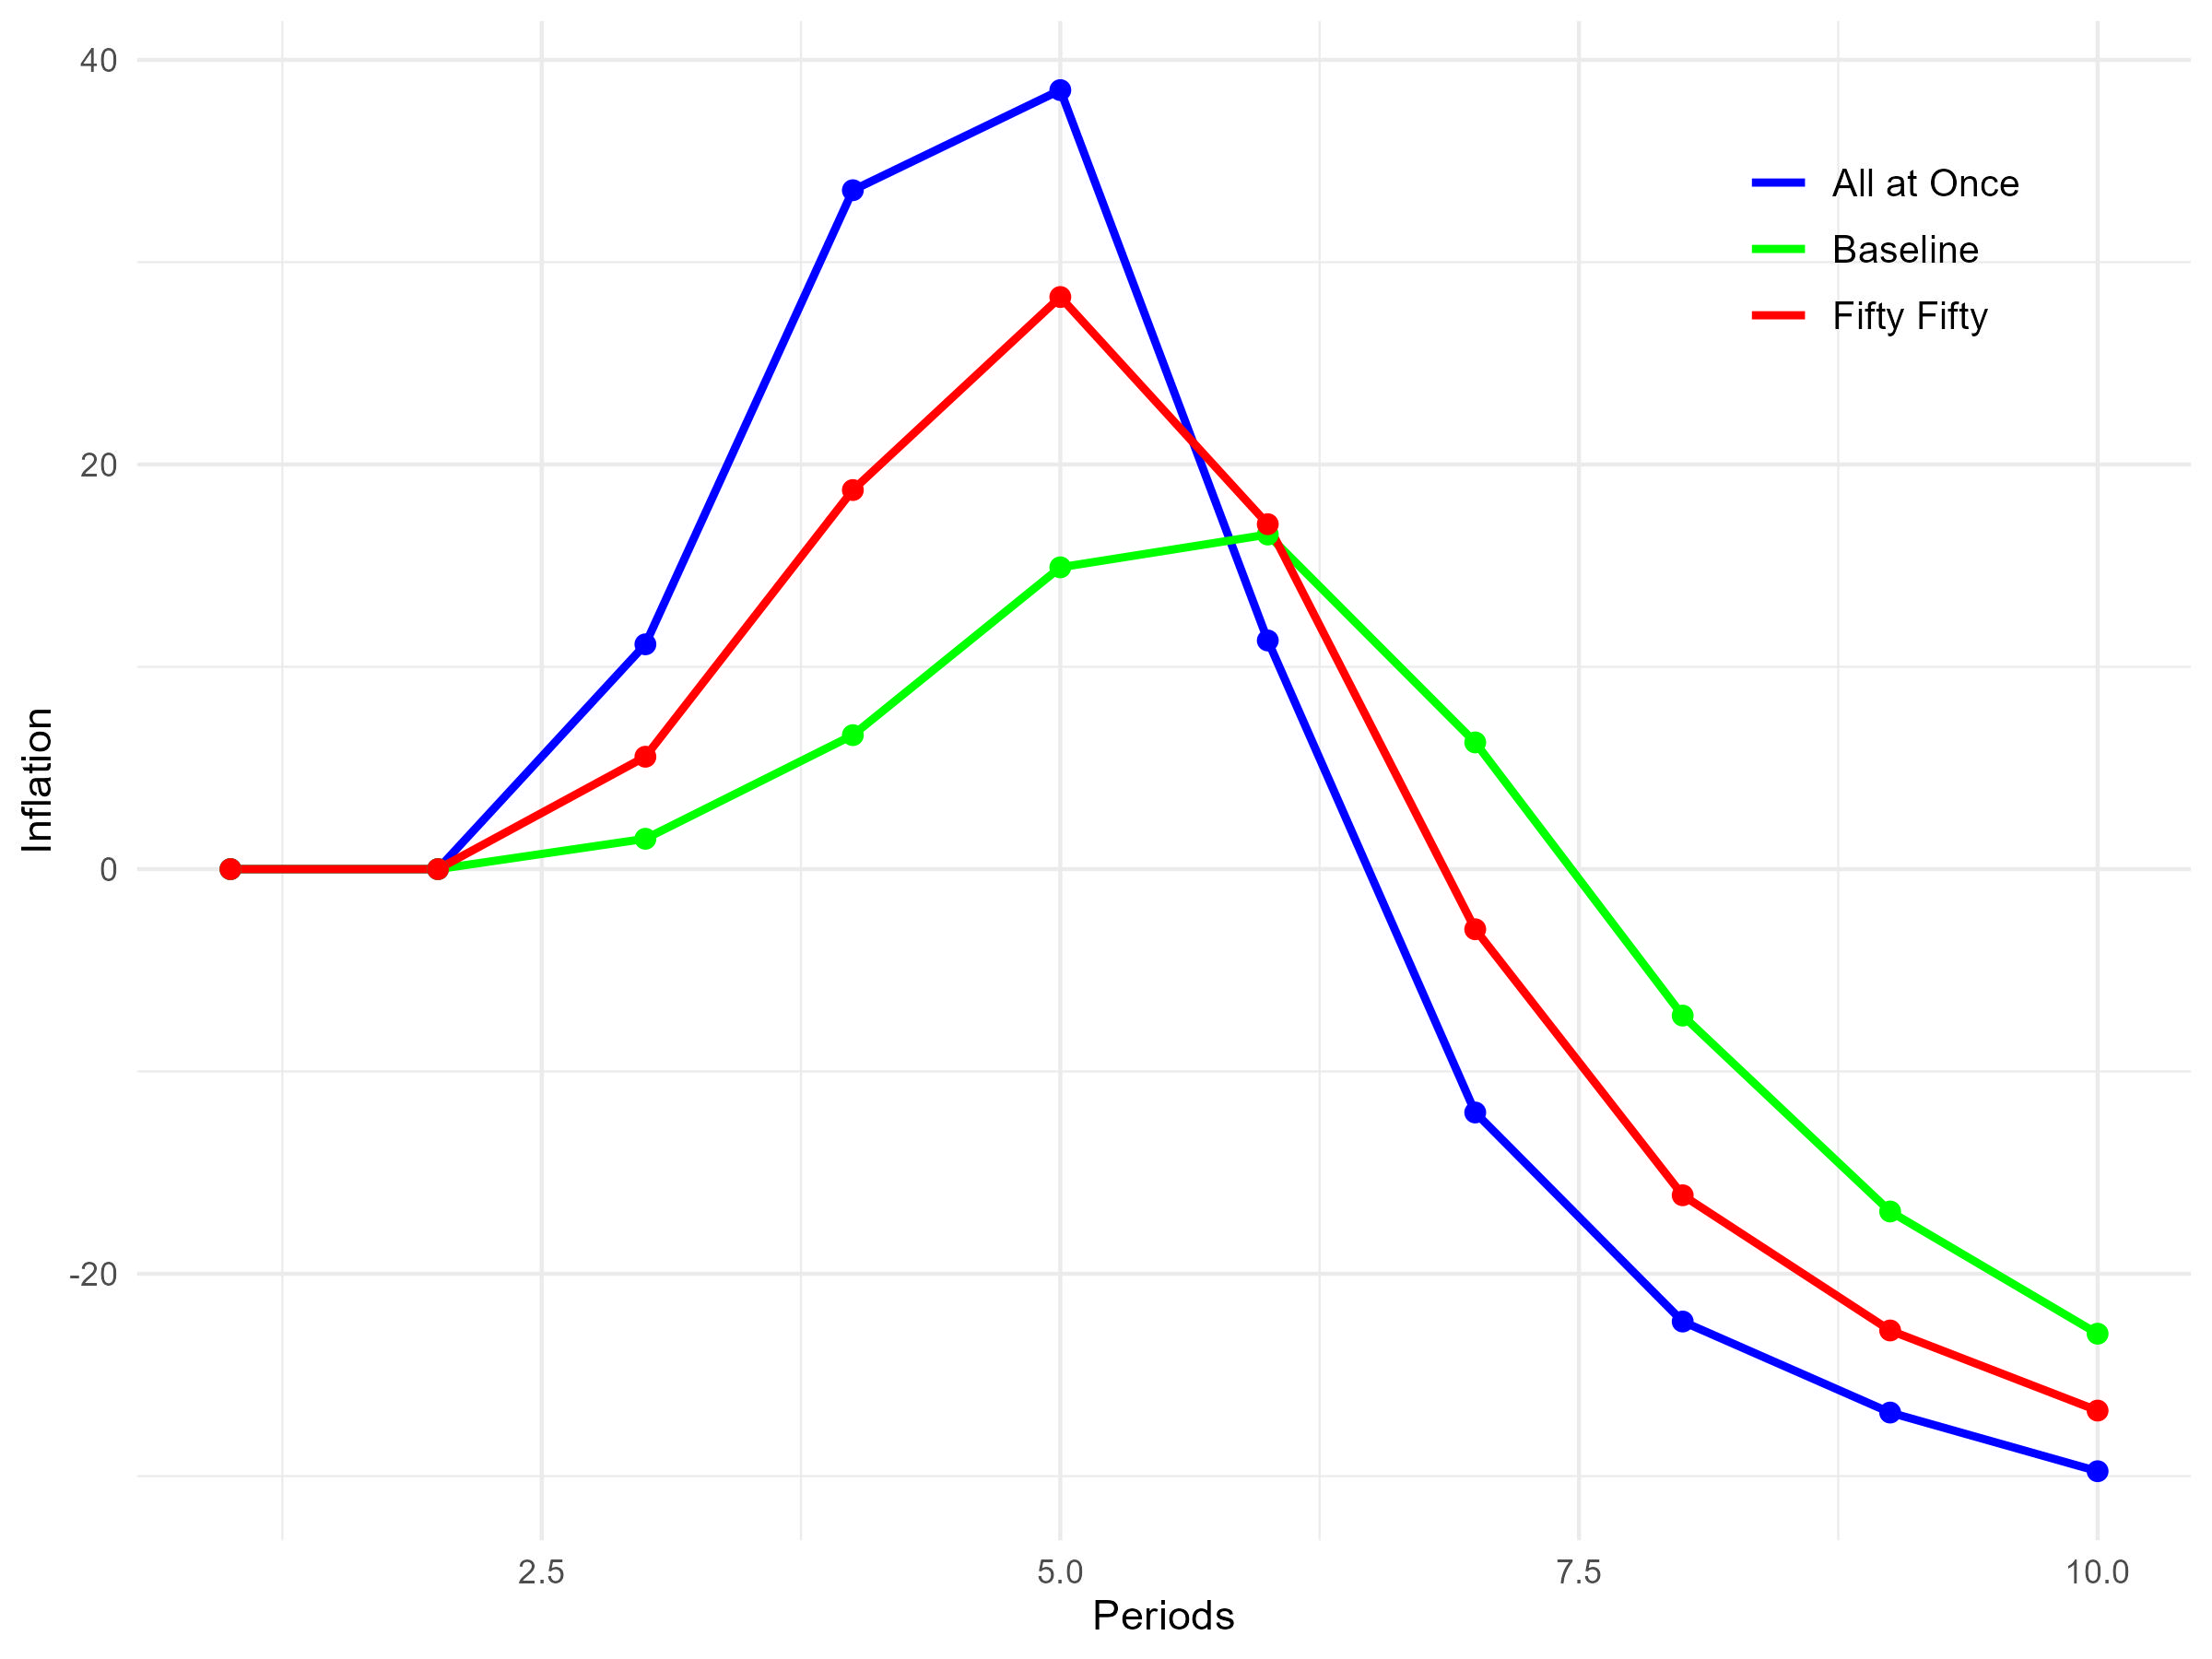
\includegraphics[width=.75\textwidth]
    {Comparing_Inflation.jpg}
    \caption{Inflation Rates Compared}
    \label{fig:Inflation Rates Compared}
\end{figure}

\begin{figure}[p]
    \centering
    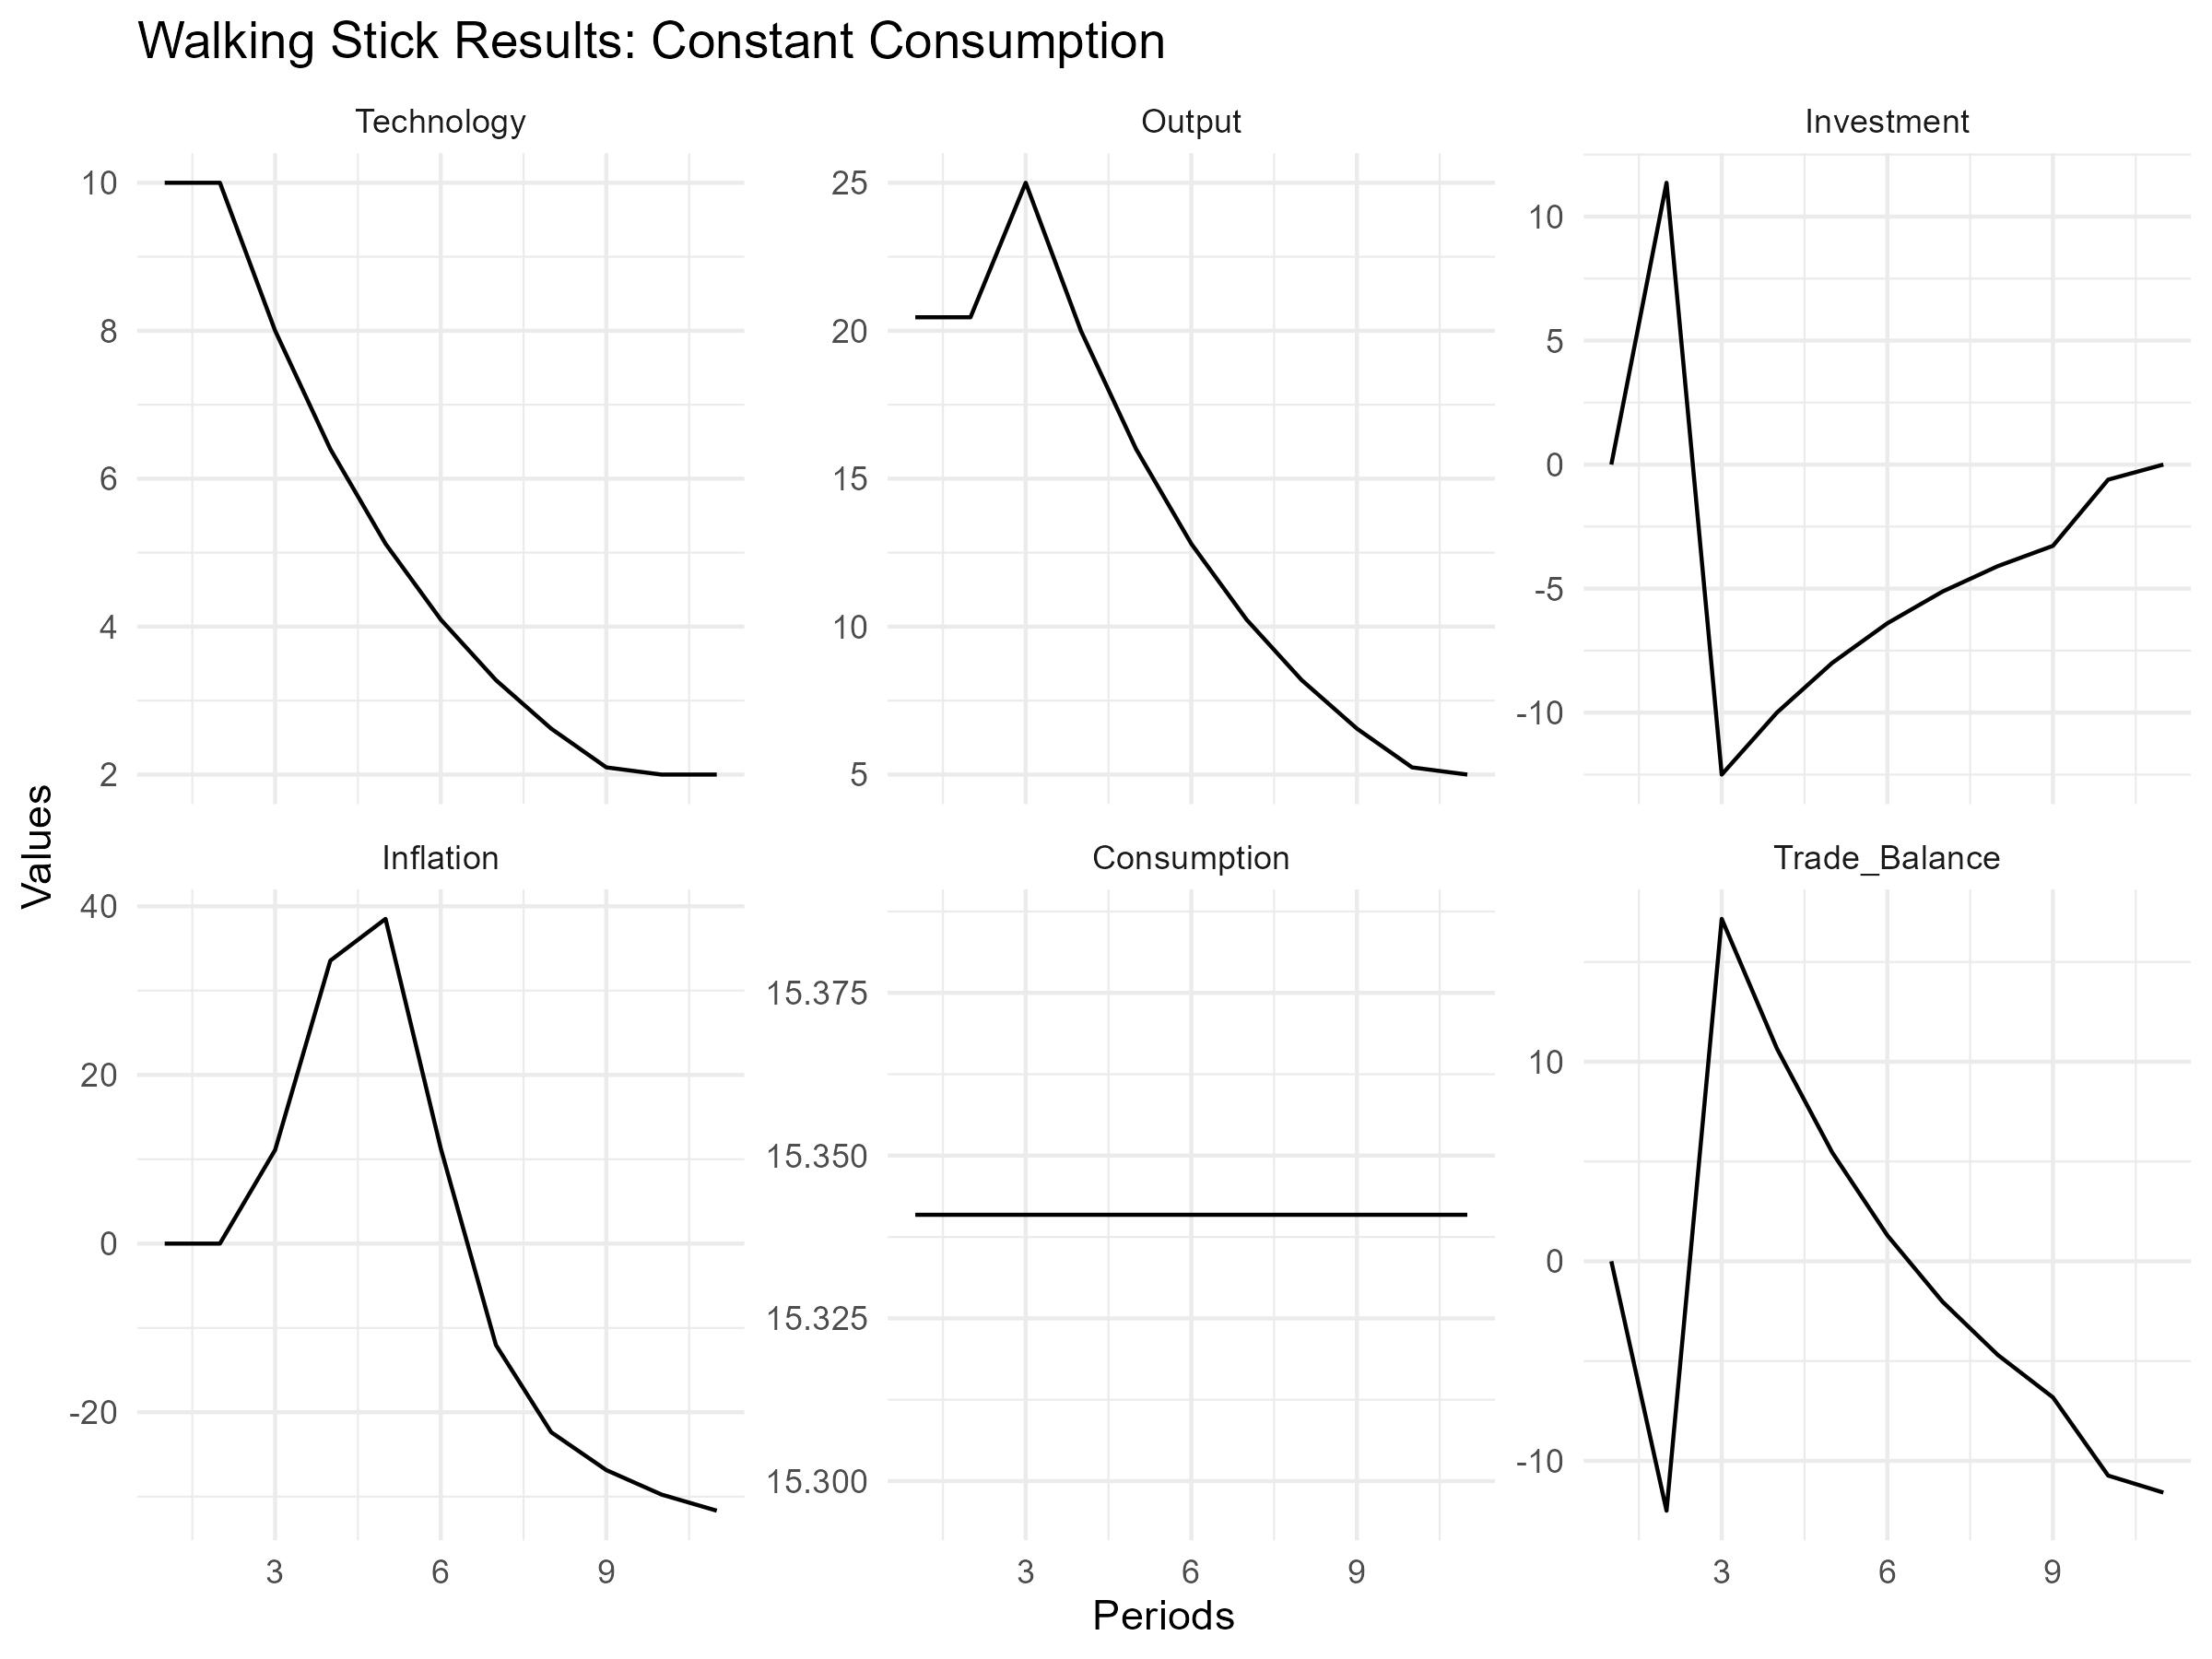
\includegraphics[width=0.75\textwidth]
    {1_All_Once_Main_Variables.jpg}
    \caption{All At Once: Main Variables}
    \label{fig:All at Once Main Variables}
\end{figure}

\begin{figure}[p]
    \centering
    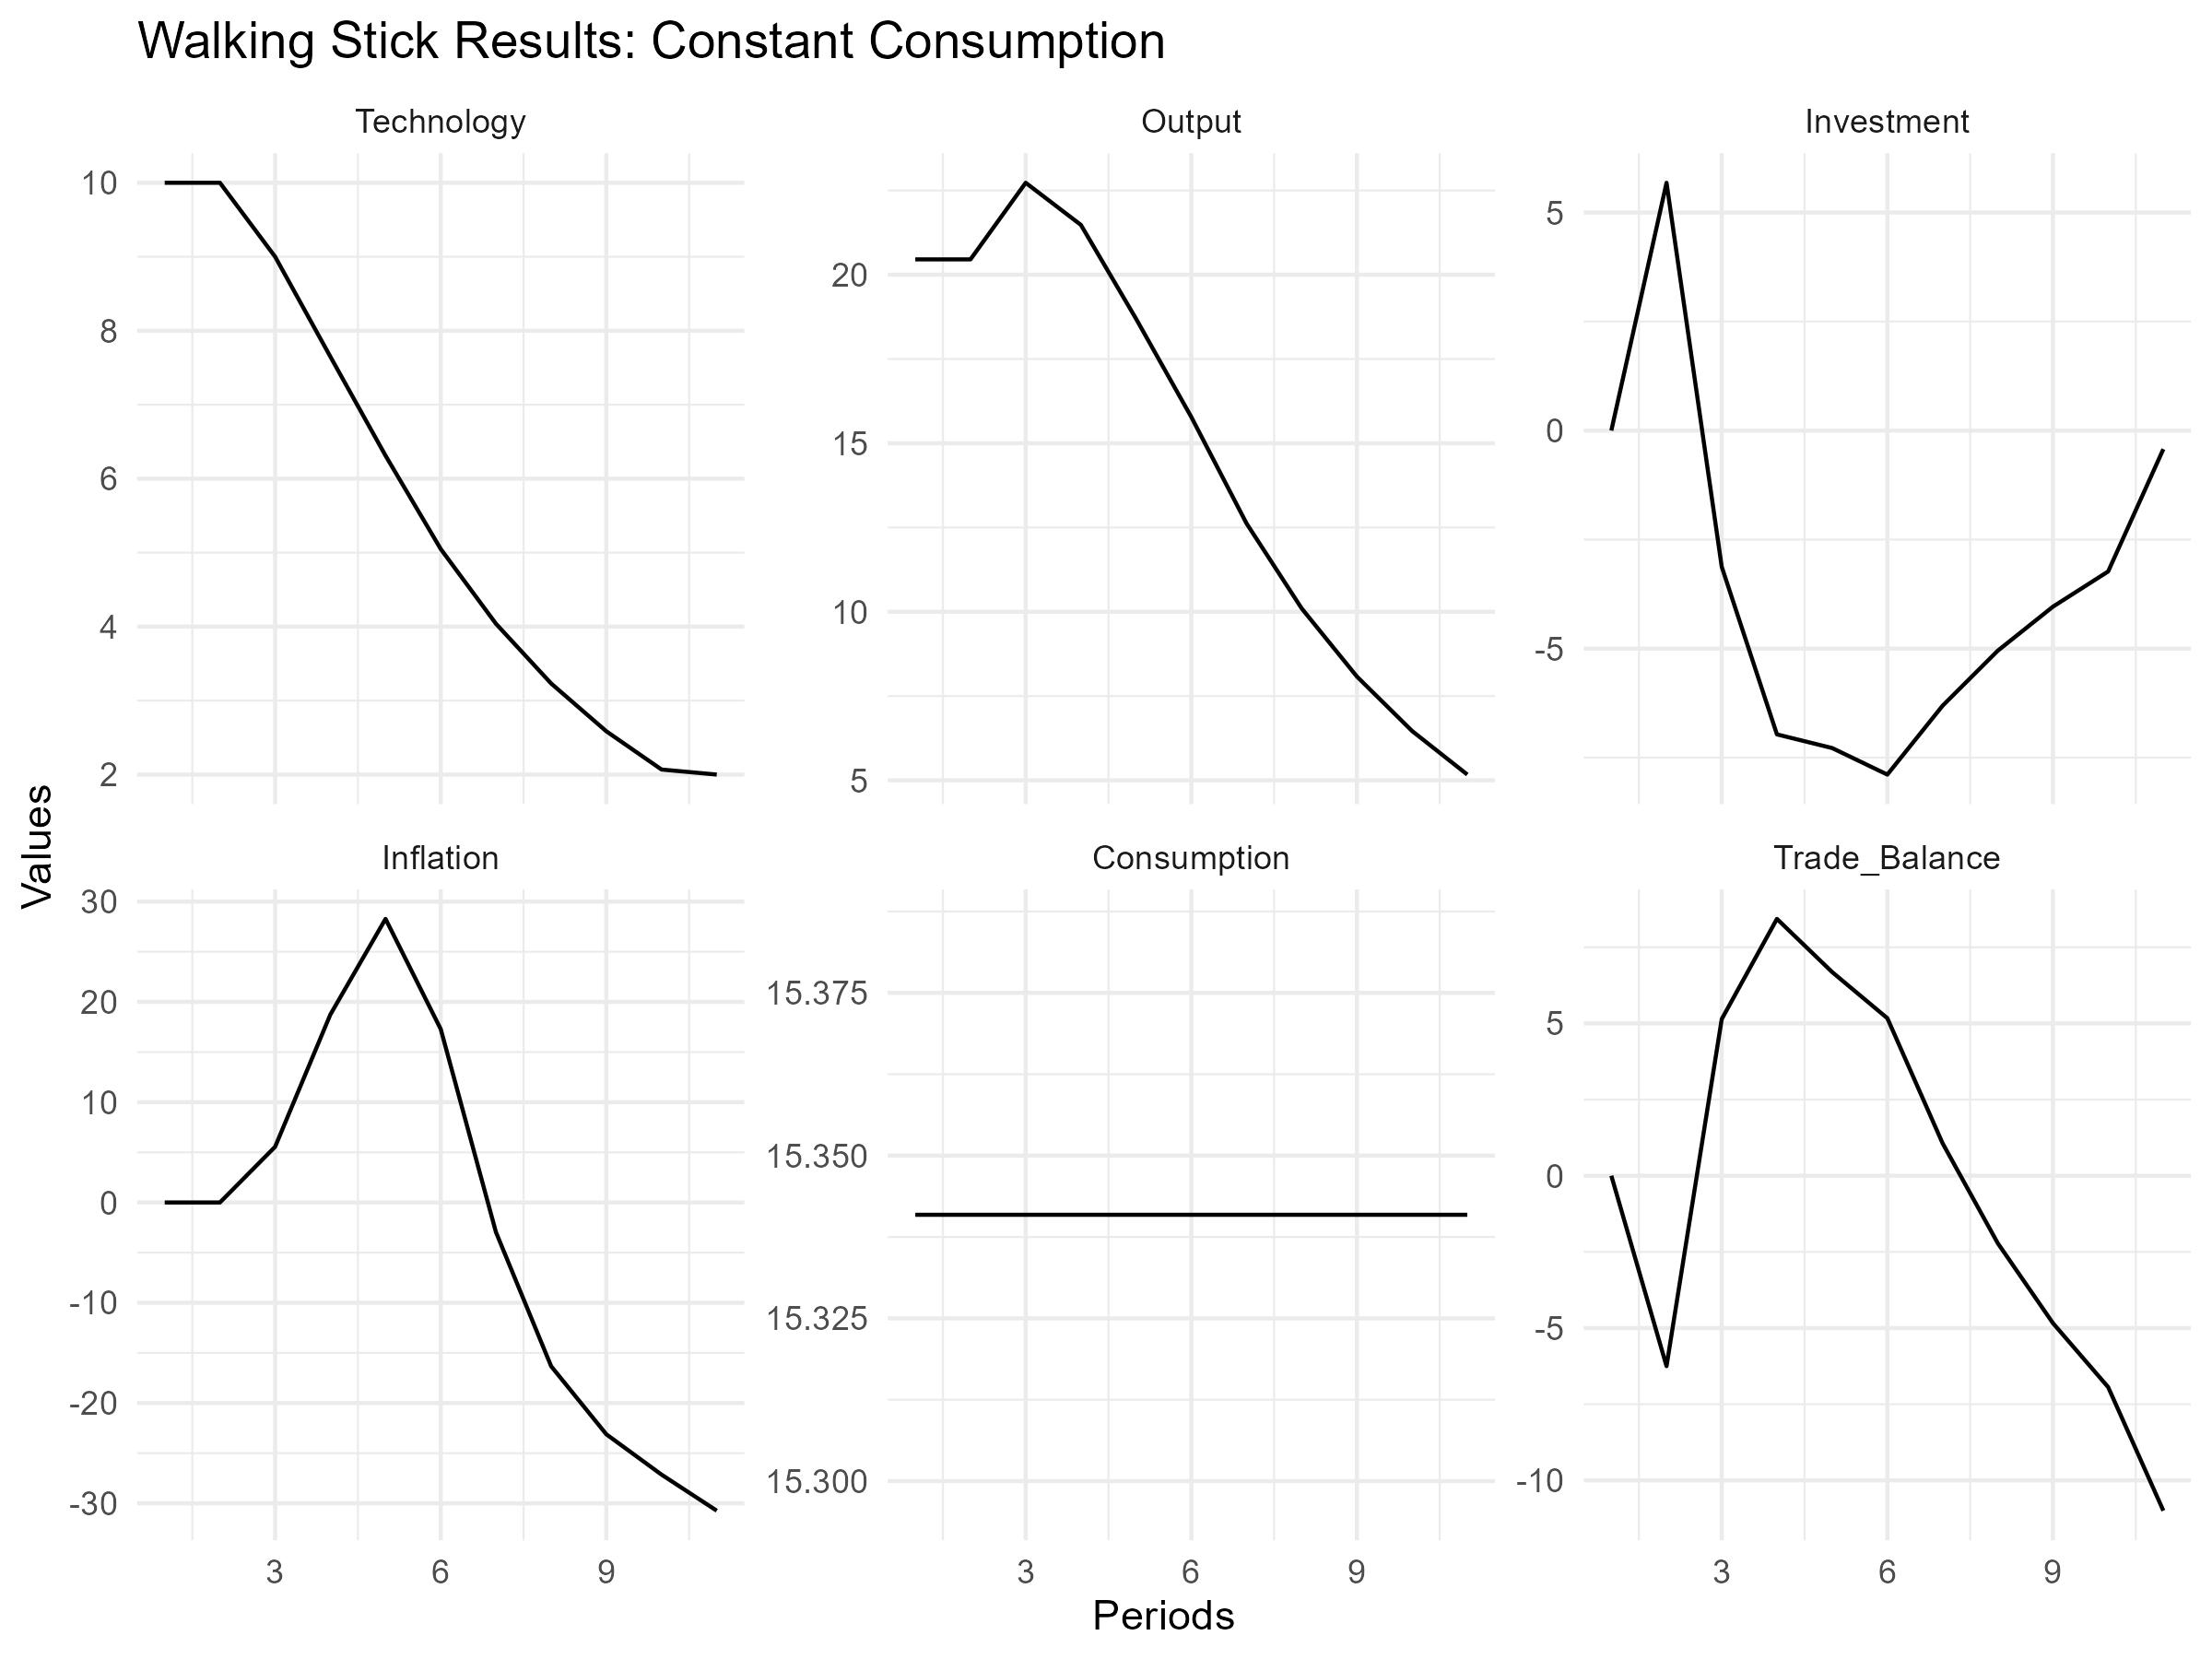
\includegraphics[width=0.75\textwidth]
    {2_50_50_Main_Variables.jpg}
    \caption{50-50: Main Variables}
    \label{fig:50_50 Main Vars}
\end{figure}

\begin{table}[h]
    \centering
    \caption{Populist Leaders Mix of \cite{FunkeEtAl2023} and \cite{BallFreytag2019}}
    \renewcommand{\arraystretch}{0.5} % Reduce row spacing
    \resizebox{.75\textwidth}{!}{%
    \begin{tabular}{|c|c|c|}
    \hline
        \textbf{Country} & \textbf{Leader} & \textbf{Years} \\ \hline
Argentina    & Peron                                         & 1946–1955    \\
Argentina    & Peron                                         & 1973–1974    \\
Argentina    & Martinez                                      & 1974–1976    \\
Argentina    & Raúl Ricardo Alfonsín Foulkes                 & 1983–1989    \\
Argentina    & Carlos Saúl Menem Akil                        & 1989–1999    \\
Argentina    & Néstor Carlos Kirchner Ostoić                 & 2003–2007    \\
Argentina    & Cristina Fernández de Kirchner                & 2007–2015    \\
Bolivia      & Hernán Siles Zuazo                            & 1982–1985    \\
Bolivia      & Jaime Paz Zamora                              & 1989–1993    \\
Bolivia      & Evo Morales                                   & 2006–2019    \\
Brazil       & Vargas                                        & 1930-1945    \\
Brazil       & Vargas                                        & 1951-1954    \\
Brazil       & Fernando Affonso Collor de Mello              & 1990–1992    \\
Brazil       & Jair Bolsonaro                                & 2019–2022    \\
Bulgaria     & Borisov I ('09-12), II ('14-17), III ('17-20) & 2009-2021    \\
Chile        & Ibanez                                        & 1927-1931    \\
Chile        & Ibanez                                        & 1952-1958    \\
Chile        & Patricio Aylwin Azócar                        & 1990–1994    \\
Colombia     & Belisario Antonio Betancur Cuartas            & 1982–1986    \\
Colombia     & Álvaro Uribe Vélez                            & 2002–2010    \\
Ecuador      & Velasco                                       & 1968-1972    \\
Ecuador      & Rodrigo Borja Cevallos                        & 1988–1992    \\
Ecuador      & Abdalá Jaime Bucaram Ortiz                    & 1996–1997    \\
Ecuador      & Lucio Edwin Gutiérrez Borbua                  & 2003–2005    \\
Ecuador      & Rafael Correa Delgado                         & 2007–2017    \\
Greece       & Tsipras                                       & 2015-2019    \\
Guatemala    & Otto Pérez Molina                             & 2012–2015    \\
Hungary      & Viktor Orbán                                  & 2010–2025    \\
India        & Narendra Modi                                 & 2014–2025    \\
Israel       & Netanyahu                                     & 1996-1999    \\
Israel       & Netanyahu                                     & 2009-2025    \\
Italy        & Silvio Berlusconi                             & 1994-1995    \\
Italy        & Silvio Berlusconi                             & 2001–2006    \\
Italy        & Silvio Berlusconi                             & 2008–2011    \\
Italy        & Lega/M5S                                      & 2018-2020    \\
Japan        & Koizumi                                       & 2001-2006    \\
Mexico       & Cardenas                                      & 1934-1940    \\
Mexico       & Luis Echeverría                               & 1970–1976    \\
Mexico       & López Portillo                                & 1977–1982    \\
Mexico       & Andrés Manuel López Obrador                   & 2018–2024    \\
Nicaragua    & Sandinistas                                   & 1979–1985    \\
Nicaragua    & José Daniel Ortega Saavedra                   & 1985–1990    \\
Nicaragua    & José Daniel Ortega Saavedra                   & 2007–present \\
Paraguay     & Fernando Armindo Lugo Méndez                  & 2008–2012    \\
Peru         & Fernando Belaúnde Terry                       & 1979–1985    \\
Peru         & Alan Gabriel Ludwig García Pérez              & 1985–1990    \\
Peru         & Alberto Kenya Fujimori                        & 1990–2000    \\
Peru         & Alejandro Celestino Toledo Manrique           & 2001–2006    \\
Peru         & Alan Gabriel Ludwig García Pérez              & 2006–2011    \\
Peru         & Ollanta Moisés Humala Tasso                   & 2011–2016    \\
Philipines   & Estrada                                       & 1998-2001    \\
Philippines  & Rodrigo Duterte                               & 2016–2022    \\
Poland       & Law and Justice (PiS)                         & 2005–2007    \\
Poland       & Law and Justice (PiS)                         & 2015-2023    \\
Slovakia     & Meciar I (1992-94), II (1994-98)              & 1992-1998    \\
Slovakia     & Robert Fico                                   & 2006–2010    \\
Slovakia     & Robert Fico                                   & 2012–2018    \\
Slovakia     & Robert Fico                                   & 2023–present \\
South Africa & Zuma                                          & 2009-2018    \\
Taiwan       & Chen                                          & 2000-2008    \\
Thailand     & Thaksin Shinawatra                            & 2001–2006    \\
Thailand     & Yingluck Shinawatra                           & 2011–2014    \\
Turkey       & Recep Tayyip Erdoğan                          & 2003–present \\
USA          & Donald J. Trump                               & 2017–2020    \\
USA          & Donald J. Trump                               & 2025-present \\
Venezuela    & Carlos Andrés Pérez Rodríguez                 & 1974–1978    \\
Venezuela    & Carlos Andrés Pérez Rodríguez                 & 1989–1993    \\
Venezuela    & Hugo Rafael Chávez Frías                      & 1999–2013    \\
Venezuela    & Nicolás Maduro                                & 2013–2025  \\ \hline
    \end{tabular}%
    }
    \label{List of Populist Leaders}
\end{table}




\bibliographystyle{ejbib}

\bibliography{References}



\end{document} 